\documentclass[12pt]{article}
\usepackage{bbm}
\usepackage{xifthen}
\usepackage{wrapfig}
\usepackage{adjustbox}
\usepackage{array}

\newcolumntype{R}[2]{%
    >{\adjustbox{angle=#1,lap=\width-(#2)}\bgroup}%
    l%
    <{\egroup}%
}
\newcommand*\rot[2]{\multicolumn{1}{R{#1}{#2}}}

\usepackage[hidelinks]{hyperref}
\usepackage{amsmath}
\usepackage{amssymb}
\usepackage{amsfonts}
\usepackage{dsfont}
\usepackage{url}
\usepackage[a4paper,left=1in,top=1in,right=1in,bottom=1in,nohead]{geometry}
\usepackage[round]{natbib}
\usepackage{multirow}
\usepackage{algpseudocode}
\usepackage{algorithm}
\usepackage{subcaption}


\newcommand{\query}{q}
\newcommand{\strsent}{s}
\newcommand{\strsents}{\mathcal{S}}
\newcommand{\nugget}{n}
\newcommand{\extract}{a}
\newcommand{\salience}{y}
\newcommand{\Salience}{Y}
\newcommand{\similarity}{k}
\newcommand{\Similarity}{K}
\newcommand{\updates}{\mathcal{U}}
\newcommand{\nuggets}{\mathcal{N}}
\newcommand{\exemplars}{\mathcal{E}}



\newcommand{\tfidf}{tf-idf }





\newcommand{\poi}{T}



\let\emph\relax % there's no \RedeclareTextFontCommand
\DeclareTextFontCommand{\emph}{\bfseries\em}










\title{\textbf{What to Write and How to Write It}\\
       \textit{\large Modeling Content Selection and Generation for Text Summarization}\\
       ~\\
       ~\\\large\textbf{Thesis Proposal}}
\author{~\\
        \textbf{Chris Kedzie}\\
        Department of Computer Science\\
        Columbia University\\
        \url{kedzie@cs.columbia.edu}}

\date{December $10^{\textrm{th}}$, 2018}

\begin{document}

\pagenumbering{gobble}
\maketitle

\pagebreak

\renewcommand{\thepage}{\roman{page}}
\setcounter{page}{1}

\begin{abstract}
Automatic text summarization is a long standing NLP problem that has recently 
seen an uptick in interest due to flexible, high capacity deep learning based 
sequence-to-sequence transduction models. 
While many researchers are turning to complex neural networks to perform
end-to-end summary generation, we argue that this unnecessarily obscures
the underlying sub-tasks for summarization. Instead, we propose an alternative
research agenda, focusing on two key summarization subtasks: 
\textit{i)} estimating the general importance of text content for summary 
inclusion, and \textit{ii)} generating text that is faithful, a notion we 
formally define, to said important content. With respect to problem \textit{i)}
we propose several novel methods for working in both low context, streaming
news scenarios, as well as, standard single document summarization settings,
including feature-based and deep learning models of content importance.
On the latter problem, we study the utility of using extractive 
summarization algorithms as a preprocessing stage for a sequence-to-sequence 
based abstractive summarizer, and finally introduce a novel algorithm for
generating text that is faithful, i.e. respects prior beliefs about structured 
knowledge in a database, in an effort to provide stronger guarantees 
about summary reliability.
\end{abstract}

\pagebreak

\tableofcontents
\newpage




\renewcommand{\thepage}{\arabic{page}}
\setcounter{page}{1}



% Change to false to compile full document.
\def\highlevel{true}

%%% Latex Table Column Types %%%

\newcolumntype{g}{>{\columncolor{black!5}}c}
\newcolumntype{f}{>{\columncolor{black!5}}r}
\newcolumntype{L}[1]{>{\raggedright\let\newline\\\arraybackslash\hspace{0pt}}m{#1}}
\newcolumntype{R}[2]{%
    >{\adjustbox{angle=#1,lap=\width-(#2)}\bgroup}%
    l%
    <{\egroup}%
}
\newcommand*\rot[2]{\multicolumn{1}{R{#1}{#2}}}

%%% General Math Notation %%%

\newcommand{\fdef}[3]{#1 : #2 \rightarrow #3}
\newcommand{\R}{\mathbb{R}}
\newcommand{\Rnonneg}{\mathbb{R}^{\ge 0}}
\newcommand{\N}{\mathbb{N}}
\newcommand{\Npos}{\N^{+}}
\newcommand{\Rn}[1]{\R^{#1}}
\newcommand{\Ind}[1]{\mathbbm{1}\{ #1 \}}
\newcommand{\Idx}[1]{\llbracket #1 \rrbracket}
\newcommand{\Sze}[1]{| #1 |}
\newcommand{\E}{\mathbb{E}}
\newcommand{\entropy}{H} 
\newcommand{\dataset}{\mathcal{D}}
\newcommand{\objective}{\mathcal{L}}
\newcommand{\discSet}{\mathcal{X}}

%%% General Lang Processing %%%

\newcommand{\tfidf}{TF-IDF}
\newcommand{\idf}{IDF}
\newcommand{\meteor}{\textsc{Meteor}}
\newcommand{\rouge}{\textsc{Rouge}}
\newcommand{\rougeN}[1]{\textsc{Rouge-{#1}}}


%%% Feature Based Salience Models Macros $$$

\newcommand{\query}{q}
\newcommand{\Queries}{\mathcal{Q}}
\newcommand{\strsent}{s}
\newcommand{\sentvec}{\mathbf{s}}
\newcommand{\strsents}{\mathcal{S}}
\newcommand{\feats}{\phi}
\newcommand{\nugget}{n}
\newcommand{\Nuggets}{\mathcal{N}}
\newcommand{\nuggets}{\mathcal{N}}
\newcommand{\predNuggets}{\hat{\Nuggets}}
\newcommand{\extract}{a}
\newcommand{\salience}{y}
\newcommand{\predSalience}{\hat{y}}
\newcommand{\saliences}{\mathbf{\salience}}
\newcommand{\predSaliences}{\mathbf{\hat{\salience}}}
\newcommand{\salThresh}{\lambda_1}
\newcommand{\simThresh}{\lambda_2}

\newcommand{\gp}{\mathcal{GP}}


\newcommand{\Salience}{Y}
%\newcommand{\similarity}{k}
\newcommand{\Similarity}{\mathbf{K}}
\newcommand{\updates}{\mathcal{U}}
\newcommand{\update}{u}
\newcommand{\exemplars}{\mathcal{E}}
\newcommand{\similarity}[2]{\textsc{Similarity}(#1, #2)}
\newcommand{\sapcluster}[2]{\textsc{AffinityPropagation}(#1, #2)}


\newcommand{\comprehensiveness}{\textsc{Comprehensiveness}}
\newcommand{\expectedGain}{\E\left[\textsc{Gain}\right]}
\newcommand{\comp}{\textsc{Comp.}}
\newcommand{\fmeasure}{F1}

\newcommand{\sap}{\textsc{Sap}}
\newcommand{\ap}{\textsc{Ap}}
\newcommand{\ranksal}{\textsc{Rs}}
\newcommand{\hac}{\textsc{Hac}}

\newcommand{\modelLS}{\textsc{L2s}}
\newcommand{\modelLSCos}{\textsc{L2sCos}}
\newcommand{\modelCos}{\textsc{Cos}}

%\newcommand{\poi}{T}


%%% Faithful Generation Macros %%%
    \newcommand{\evidence}{x}
    \newcommand{\evidenceSpace}{\mathcal{X}}
    \newcommand{\evidenceSpaces}[1]{\evidenceSpace_1
    \times \cdots \times \evidenceSpace_{#1}}
    \newcommand{\utterance}{y}
    \newcommand{\gen}{p}
    \newcommand{\genParams}{\theta}
    \newcommand{\rec}{q}
    \newcommand{\recParams}{\phi}
    \newcommand{\vocab}{\mathcal{V}}
    \newcommand{\faithful}{\textsc{Faithful}}


\newcommand{\beamDistr}{\beta}


%%% Learning To Summarize
\newcommand{\policy}{\pi}
\newcommand{\policySpace}{\prod}
\newcommand{\lsAction}{a}
\newcommand{\lsActionSpace}{\mathcal{A}}
\newcommand{\oraclePolicy}{\policy^{*}}
\newcommand{\modelPolicy}{\hat{\policy}}
\newcommand{\rollOutPolicy}{\policy^{out}}
\newcommand{\lsState}{s}
\newcommand{\lsStateSpace}{\mathcal{S}}
\newcommand{\lsStep}{t}
\newcommand{\lsTrans}{T}
\newcommand{\lsSaliences}{\mathbf{y}}
\newcommand{\lsSaliencesRollOut}{\mathbf{y}}
\newcommand{\lsSaliencesRef}{\mathbf{y}^*}
\newcommand{\lsStrucLoss}{\ell}
\newcommand{\lsCost}{c}
\newcommand{\lsChoiceParam}{\beta}
\newcommand{\policyParams}{\mathbf{W}}
\newcommand{\lsFeats}{\phi}

%%% Deep Learning Models of Content Salience %%%

\newcommand{\sent}{s}
\newcommand{\Sents}{\mathcal{S}}
\newcommand{\doc}{d}
\newcommand{\lbl}{y}
\newcommand{\Labels}{\mathbf{y}}
\newcommand{\word}{w}
\newcommand{\extracts}{\mathcal{E}}
\newcommand{\budget}{c}
\newcommand{\encoder}{\textsc{Encoder}}
\newcommand{\extractor}{\textsc{Extractor}}
\newcommand{\embproj}{W}
\newcommand{\emb}{\omega}
\newcommand{\embsize}{n}
\newcommand{\sembsize}{m}
\newcommand{\semb}{\mathbf{h}}
\newcommand{\rsemb}{\overrightarrow{\semb}}
\newcommand{\lsemb}{\overleftarrow{\semb}}
\newcommand{\gru}{\textsc{Gru}}
\newcommand{\rgru}{\overrightarrow{\gru}}
\newcommand{\lgru}{\overleftarrow{\gru}}
\newcommand{\cfeat}[2]{\mathbf{f}_{#1}^{( #2 )}}
\newcommand{\relu}{\textsc{ReLU}}
\newcommand{\winsize}{k}
\newcommand{\winsizes}{K}
\newcommand{\fmapsize}{F}
\newcommand{\cfidx}{l}
\newcommand{\cact}{a^{(\cfidx,\winsize)}}
\newcommand{\cnnbias}{\mathbf{u}^{(\winsize)}}
\newcommand{\cnnweight}{\mathbf{U}^{(\winsize)}}
\newcommand{\cnnBiasSpace}{\mathbb{R}^{\fmapsize_\winsize}}
\newcommand{\cnnWeightSpace}{\mathbb{R}^{\winsize \times \fmapsize_\winsize \times \embsize}}

\newcommand{\extHid}{\mathbf{z}}
\newcommand{\rExtHid}{\overrightarrow{\extHid}}
\newcommand{\lExtHid}{\overleftarrow{\extHid}}
\newcommand{\demb}{\mathbf{d}}
\newcommand{\smemb}{\mathbf{s}}
\newcommand{\posemb}{\mathbf{f}}
\newcommand{\qrtemb}{\mathbf{c}}

\newcommand{\enextHid}{\mathbf{e}}
\newcommand{\deextHid}{\mathbf{d}}


%%sent enc
\newcommand{\enAvg}{\textsc{Avg}}
\newcommand{\enRnn}{\textsc{Rnn}}
\newcommand{\enCnn}{\textsc{Cnn}}

%%% Wimpy Models %%%
\newcommand{\elmo}{\textsc{Elmo}}
\newcommand{\glove}{\textsc{Glove}}

\newcommand{\bowvec}{\omega}

\section{Introduction}

Everyday we ask friends and colleagues to do it, to tell us about books, 
newspaper articles, and other complex pieces of text, and, without more than a 
moment's reflection, they are able to compress their experience
into succint statements in natural language that adequately sum up the thing
being described. The ease with which we summarize belies the difficulty in 
writing programs that do so automatically, and so it would appear that 
the robust
ability to create summaries is, as of 2018, a uniquely human capability.
This partially explains its allure to the artificial intelligence (AI)
research community, which has in one way or another, attempted to aggregate
and naturally compress text data since at least the 1950's 
\citep{luhn1958automatic}.
This makes automatic text summarization one of the longest-standing 
application areas in the 
field of natural language processing (NLP), with a history as long and varied
as some of the more foundational tasks, e.g. parsing and tagging. 

While there are many variants, 
the general summarization task is 
to reduce a large input text into its most essential pieces of information,
and in doing so reduce the amount of reading a human has to do. 
In this thesis we focus on advances to two summarization subtasks:
\textit{(i)} identifying the most import content for inclusion in the summary, 
and \textit{(ii)}
rendering that content in such a way as to not misrepresent the original 
input. We refer to the former as \emph{salience estimation} and the latter
as \emph{faithful generation}. 

The completed and proposed methods of salience estimation cover a range of
techniques including feature-based regression, clustering, learning-to-search,
and deep learning. We experimentally verify the utility of our approaches
across a variety of summarization tasks including stream summarization,
single-document summarization, and multi-document summarization.
The general research goal here is to develop flexible models for 
identifying
important words, phrases, and sentences that are likely to serve as 
representitive members of the larger text in which they are found.

In \emph{extractive summarization}, 
where the summary is constructed by copying and pasting phrases or sentences 
from the input text, salience estimation can be used directly to create
a summary. For example, a simple method of sentence extractive summarization
would be to order the input sentences in decreasing salience and select the
top few sentences for the summary. In most cases, salience is not the only
consideration for summary inclusion; redundancy, discourse coherence, fluency,
and many other metrics of text quality can and have been used as content
selection criteria. These measures are largely independent of salience 
(with the noteable exception of redundancy) and so we do not explore them in 
detail here). Our salience estimation methods will constitute the bulk of the
proposed thesis, the details of completed and proposed work can be found
in \autoref{sec:chapter3} and \autoref{sec:chapter4}.

In \autoref{sec:chapter3} we develop two feature-based models of sentence
salience and evaluate them in a relatively novel \emph{stream summarization} 
crisis-monitoring scenario
\citep{starbird2013working,aslam2016trec}. In this task, a user is interested
in tracking information about a disaster event (e.g. a hurricane). The
user provides a text based query describing the event 
(e.g. ``Hurricane Sandy'') and the summarization model must then 
monitor a stream of news articles, identifying important sentences in the 
document stream and presenting them to the user. The information must be 
highly salient to the query event, as well as novel to the user, and timely
-- we do not want to bombard the user with irrelevant or repeated information,
and our methods used cannot take so long to identify content that the 
information found is out of date.
  
We develop and compare several deep learning based models of word and 
sentence salience in \autoref{sec:chapter4} and evaluate them primarily on
sentence extractive \emph{single document summarization} (SDS). 
We perform this evaluation across
a variety of genres including news, personal narratives, and medical journal
articles. Intuitively, the goal here is to summarize a single news article, 
short story, or research paper by selecting a subset of the input sentences
to serve as the summary. We also explore adaptation of these algorithms to 
the sentence extractive \emph{multi-document summarization} (MDS) task, 
where there is much less data, and only in the news genre.
This is similarly straightforward, given a set of related news articles 
(typically ten), select a subset of the sentences to use as the summary of
the document set.


Salience estimation can also be used to guide 
\emph{abstractive summarization} techniques, i.e. methods that produce novel
summary text using a generative model. These types of models 
must (at the very least) implicitly select important content for conditioning 
their
generative process, and salience estimation can be used for precisely this 
purpose. 

Research in abstractive summarization is increasing, in part due to
the success of general purpose sequence-to-sequence transduction models 
in machine translation (MT) that have been ported to the summarization task.
The ability of abstractive models to generate relatively fluent and 
meaningful summaries is impressive. However, they are also especially prone 
to generating generic statements that are not grounded by evidence in the 
input. This seems to be a well known problem among researchers working
in generation, but it has not received much attention in the literature.
We are interested in this problem from both the perspectives of selecting
the right evidence in the input for generation, a task for which we enlist
our salience estimation methods, and also certifying that a generated text
conforms to knowledge represented in the input or possesed by the model
apriori. For the latter goal, we propose to model generation as a two player
game, where one player, the generator, is tasked with producing a text
utterance describing a piece of evidence (either text or structured data);
the second player, the recognizer, %change this name
evaluates the plausibility of the utterance with respect to the evidence.
This overall regime will consitute our method of faithful generation,
to be outlined in more detail in \autoref{sec:chapter5}. We propose 
evaluation both on an SDS task, as well as, a data-to-text generation 
test bed \citep{wiseman2017challenges}.

\subsection{Contributions}

To summarize, our comleted and proposed contributions of this thesis are as 
follows:
\begin{enumerate}

 \item Two novel feature-based models of sentence salience and an empirical
    evaluation in a stream summarization task.
% \item A novel approach to streaming summarization using a feature-based
%     regression model of sentence salience and sentence selection using 
%     exemplar-based clustering.

% \item A novel approach to streaming summarization using the locally optimal
%     learning to search (LOLS) algorithm.

 \item Several novel deep learning architectures for word and sentence 
   salience, as well as a thorough evaluation of the linguistic and
   structural features critical to learning in the SDS task across a 
   variety of genres.

 \item Adaptation of the deep learning based SDS models to a news MDS task. 

 \item A novel training regime for generative models of text to ensure
          faithfulness of text output to structured data or 
         prior distributions over structured data.

 \item A novel method of combining salience estimation based extractive 
     summarization with abstractive generation in the faithful generation
    paradigm.    

%An experimental evaluation of several existing and novel deep learning
%   architectures for word and sentence salience with 
%A study on the design, strengths, and limitations of deep learning 
%     models for content selection at the sentence and word level in 
%     single document summarization. 

% \item An experimental study of extractive content selection algorithms
%     as input to abstractive summarization model.

% \item A novel approach to generating text that is faithful to some
%     structured information in a database.

\end{enumerate}




%The first two contributions focus broadly on estimating content importance
%or salience for various summarization tasks and domains. They further
%can be broken down into traditional feature-based models (the first two 
%contributions) and deep learning models (the third contribution).
%The last two contributions focus on generating text from previously 
%selected content, with the fourth contribution studying the case where
%selected content consists of extracted sentences and words from an input
%document, and the final contribution focuses on generating text that is 
%faithful to some structured information. 

Together, these contributions
provide a recipe book for identifying summary worthy information and 
generating text that respects truth statements about that information.
The hope is that these methods will lead to more reliable summaries
without sacrificing the expressiveness of the generation algorithm. 

In the next section we describe related work (Section 2). Section 3 describes
completed work on the feature-based approaches to sentence salience estimation.
In section 4, we describe completed and ongoing work on deep learning models
of salience estimation. We describe our planned approaches to faithful 
generation in section 5. Section 6 describes our research plan, before 
we finally conclude.





\ifthenelse{\equal{\highlevel}{false}}{\section{Related Work}


The complete range of methods and task variations covered by the summarization
literature are too numerous to describe completely here. In the space 
available, we give an overview of unsupervised and supervised learning
approaches to estimating word and sentence importance. 
We also give some background on the variety
of summarization tasks, and the manner in which they are evaluated.


\subsection{Unsupervised Word Importance}


The most obvious signal available for estimating word importance is word 
frequency, i.e. frequent word occurences (modulo stopwords) are likely 
to be related the important topics of the document or document collection 
\cite{topic_sigs}, and it is the chief ingredient in all of the following
word importance estimators.
Term weighting schemes from information retrieval
have frequently been used, most commonly tf-idf 
\cite{centroid,maybe_conroy,find_others}. 
Various probabilistic weightings have also been considered, e.g. the
observed document probability \cite{freq_sum} or the ratio of background
corpus probabiltiy to document probability \cite{topic_sigs}.
Information theoretic transformations of word frequency like the document
level term entropy
have also been found to be useful \cite{klsum,reference_less_summarization}.
Latent semantic analyis (LSA), latent dirichlet allocation (LDA), and
other matrix factorization schemes have been used to find a low dimensional
``concept'' representation for each word, the sum of the concept contributions
constituting the word importance score \cite{multiling_stuff}.
Finally, various methods of transforming word co-occurences into a word graph
have been used in conjunction with unsupervised graph ranking algorithms
\cite{lexrank,conroy_multiling,zhao_2009}.


\subsection{Unsupervised Sentence Importance}

 Graph based ranking that has been used for word importance has similarly 
been used to estimate sentence importance, where the graph consists of 
sentence vertices and edge weights are computed using pairwise sentence 
similarity \cite{textrank}. Another popular method is the centroid method
\cite{centroid} where an average vector representation for a document set is 
constructed and sentences are ranked by their similarity to the centroid object.
Sentence clustering methods have also been applied. In all these methods, 
sentences are tpyically represented as term vectors where the weights for 
each term item are determined by one of the methods mentioned in word importance
estimation methods. 


\subsection{Supervised Word Importance}

The growing availibilty of large text collections with summaries has also
encouraged the development of many supervised methods for learning the word 
importance 
directly from the data. \cite{Regsum} use many of the unsuperivsed word  
importance measures, (e.g. frequency, entropy, document position) to estimate
the probabiltiy of a word occuring in a human abstract. Learning-to-rank
has also been explored in a variety of contexts. For example in single
document summarization, \cite{lapata} used convolutional neural networks
learn rankings and while \cite{guo,macreadie} use a feature based model
to rank sentences in a streaming summarization task.
Word importance weights have also been learned in combinatorial optimization
based approaches to summarization; in several integer linear program (ILP)
formulations of the summarization problem unigram and bigram weights 
are learned \cite{gillick,martens,berkely}, in addition to learning based
submodular optimization approaches \cite{submod,svm}.




\subsection{Supervised Sentence Methods}


Structured prediction methods have also been explored. The most common is
to model the sentence selection problem as an integer linear program (ILP)
and learning typically happens in a large margin/structured svm framework 
\cite{durret}. In addition to learning ngram feature weights, discourse,
and redundancy features can also be modeled \cite{somebody}. 
Deletion based compression 
and phrase substitution have also been modeled using ILPs, where non-essential
phrases can be discarded or shortened, and entity references rewritten, e.g.
turning a pronominal reference into a nominal one.

Sentence selection can be viewed as a submodular set optimization 
(submodularity in set theory is analagous to convexity in functional analysis)
where greedy selection algorithms can efficiently find the best subset of 
sentences according to a set scoring function and budget constraints.
Learning of the scoring function has been done by \cite{uwsipos} using 
linear functions on ngram features. Feature weights can similarly be learned 
in a large margin svm framework.


Sentence selection can be modeled as a sequence tagging problem, e.g. using
hidden Markov models \cite{conroy}.

Dependencies between sentence selection can be difficult, and so in the
spirit of naive Bayes, it can be fruitful to model sentence selection as 
independent classification problems. For example, \cite{kupiec} use ....


\cite{drago_nn} use a graph convolutional neural network on top of a sentence
graph constructed from either discourse structure or sentence similarity.


Learning to rank methods have been explored, see \cite{lapata}.

\subsection{Text Generation}


While there are a variety of text generation methods, we cover three main
approaches, template based generation, sentence fusion, and 
sequence-to-sequence models.



\paragraph{Template-Based Generation} 


\paragraph{Sentence Fusion} Sentence fusion attempts to combine two or
more sentences into one. This is typically done by selecting one sentence
as the backbone, and then aligning the remaing sentences to the backbone.
Heuristics are used for backbone selection and alignment. This method
is better suited to cases where there is much redundancy between candidate
summary sentences since fusing radically different sentences is likely to
yield misleading results.
this approach is that it is difficult 



Thanks to recent advances in neural machine translation (NMT), we now
have flexible, high capacity models for generating free form text from
an arbitrary sequence input. This has led to a host of work exploring 
variety for attention based models to the summarization task \cite{everybody}.
Adaptations to attention like copying have been found to be helpful for 
handling out of vocabulary terms and controlling for repetitive outputs 
\cite{seeandothers}.
One difficulty with this approach is that is hard to control the output,
spurring additional research in more controllable neural text generation.
Length \cite{lc1,lc2}, sentiment \cite{contr}, and domain \cite{socher_I_think}
have been explored, typically by treating the feature under control 
as a learned embedding that is fed as an additional input into the generator.
\cite{lapata} explore a method similar too our faithful text generation model,
however we intend to explore some differences.




 
\subsection{Other stuff from other sections}
Estimating the salience of words and phrases is core to the problem of 
summarization. For example, \cite{luhn1958automatic} 
noted how the most topically central words in a document occur not too much 
but not
too little, and that,
``the presence in the region of highest frequency of many of the words
 previously described as too common to have the  type  of
 significance being sought would constitute
`noise' in the system.''
Typically, this has been done with heuristically derived word weights
\citep{luhn1958automatic,sparck1972statistical} or feature-based, linear 
models of sentence salience \citep{martins2009summarization,woodsend2010automatic,berg2011jointly,durrett2016learning}.

However, the recent availability of large scale single-document summarization 
data \citep{sandhaus2008new,hermann2015teaching,grusky2018newsroom}. 
With these corpora, and other developments in word embedding representation 
\citep{mikolov2013distributed,pennington2014glove},
many researchers have been developing end-to-end models of both 
abstractive \citep{rush2015neural,chopra2016abstractive,cheng2016neural,nallapati2016abstractive,see2017get,paulus2017deep} and extractive \citep{cheng2016neural,nallapati2016classify,nallapati2016summarunner,narayan2018ranking} summarization.
While the spirit of ``let a thousand architectures bloom'' has spurred much
creativity and performance gains, it has left us with little explainability
about how such models work. 

While different components of the neural architectures may be justified 
by intuition, these methods are largely black boxes and it is not clear
how they are making their sentence selection predictions. This is especially
problematic in abstractive summarization, but it is also not well understood
how extractive methods make their decisions either.




~\\
~\\





Subsequently, many methods have been proposed for salience estimation
in the context of summarization. Word weights have typically been derived
in an unsupervised way from a large collection of in-domain text.
The classic example here is Term Frequency-Inverse Document Frequency
(\tfidf) weighting \citep{sparck1972statistical}, whose aim is similar in 
spirit to Luhn's: important 
words occur frequently in the current context (the term frequency component)
 but not so much that they occur in every document 
(the inverse frequency component).

While \tfidf weights (and others like BM25 \citep{bm25}) have been frequent
ingredients in many summarization systems \citep{a,b,c,d,e}, they are 
not specifically tuned to any one summarization task. Another prominent
strand of research has been the learning of word or ngram specific weights
typically for use in linear models of salience \citep{martins2009summarization,woodsend2010automatic,berg2011jointly,durrett2016learning}. 
Given the small size of most summarization datasets at the time, one could question 
the utility of learning ngram weights when it was unlikely that there 
would be adequate data to learn broad coverage summarizers.

%In this chapter we investigate neural network architectures for extractive
%summarization, in the hopes of better understanding what is important 
%for the underlying word and sentence representations to learn.
%We start a description of completed experiments for sentence extractive
%models of summarization \citep{kedzie2018deep}, and then complete the chapter with a description
%of planned and ongoing word importance estimation techniques using deep
%learning models.


~~\\
~\\






Increasingly, researchers are returning to single document summarization,
once thought to be too difficult for automatic summarization methods.
This has been driven both by the availability of large corpora (the
most popular corpus, CNN-DailyMail, has a little over 300,000 data points
\citep{see2017get}) and by the development of general purpose 
generative models of text from the neural machine translation community.
Accordingly, the bulk of the research has used this corpus, (and the NYT
corpus \citep{sandhaus2008new}) to focus on abstractive summarization
research \citep{rush2015neural,chopra2016abstractive,cheng2016neural,nallapati2016abstractive,see2017get,paulus2017deep}. 
There has been a smaller but similar proliferation of sentence
extractive single document summarization papers on these corpora also using 
neural network architectures \citep{cheng2016neural,nallapati2016classify,nallapati2016abstractive,narayan2018ranking}.


}{}
\section{Feature-Based Models of Sentence Salience}
\label{sec:chapter3}
\label{sec:feature_salience}
We propose two novel approaches to the streaming summarization task
using biased affinity propagation (AP) clustering \citep{frey2007clustering}
and learning-to-search (L2S) \citep{daume2009search,chang2015learning}.
These models led to the publication of two papers 
\citep{kedzie2015predicting,kedzie2016real}, in addition to participation 
in the TREC Temporal Summarization tracks where we were the top performer in
2014 and the fourth and fifth place performer in 2015 
\citep{aslam2015trec,aslam2016trec}. 

In the Temporal Summarization track, the grounding scenario was disaster
summarization, where a participant system received a brief query string 
$\query$ describing a natural or man-made disaster, and the system was 
expected to process a time-ordered stream of documents relevant to the query, 
extracting sentences that were likely to contain important facts about the
event. Each query corresponded to a real-life disaster that was significant
enough to have an associated entry in Wikipedia.

For each query, human annotators also collected a reference set of important 
facts, which we refer to as \textit{nuggets}, 
from the revision history of that query's associated Wikipedia page. 
Nuggets consist of a piece of reference text and timestamp for when this piece
of information first appeared in the Wikipedia revision history. 
See \autoref{fig:eventsnuggets} for example queries and nuggets.

\begin{figure}
    \begin{tabular}{p{7.5cm}|p{7.5cm}}
         \textbf{``hurricane sandy''} &\textbf{``boston marathon bombing''} \\
        \hline
        \parbox{7.4cm}{\small
    $[\textrm{10/23 8:20pm}]$ Sandy strengthened from a tropical depression 
    into a tropical storm \\
    $[\textrm{10/23 8:20pm}]$ 2 pm Oct 23 Sandy moving north-northeast at 4 
    knots \\
    $[\textrm{10/23 8:53pm}]$ forecast track uncertain \\
    $[\textrm{10/25 12:20am}]$ In Jamaica damage was extensive
} & \parbox{7.4cm}{ \small
    $[\textrm{04/15 7:31pm}]$ Authorities are investigating a report of two 
    explosions at the finish line of the race. \\
    $[\textrm{04/15 8:29pm}]$ Some Boston Transit system service has been 
    halted.\\
    $[\textrm{04/16 12:37am}]$ Police confirmed another explosion at the JFK
    Library.
}
\end{tabular}
    \caption{Example event queries in bold, and several example nuggets below.
    Nugget timestamps are show in brackets.}
    \label{fig:eventsnuggets}
\end{figure}




We will refer to the set of extracted sentences as the update or extract
summary interchangeably. Similarly, we will use the phrases extract a sentence,
select a sentence, or emit a sentence to mean we add a sentence in the 
document stream to our rolling update summary. If a sentence $\strsent$ 
expresses the same piece of information as a nugget text $\nugget$ 
we say that $\strsent$ contains $\nugget$ or $\nugget \in \strsent$.

Systems are rewarded when they find sentences that contain important and novel
nuggets. Systems are penalized for 
selecting sentences that are irrelevant (i.e. contain no nuggets) or 
contain nuggets already covered by previous updates. 
Latency penalized metrics are also computed where
the importance of a nugget decays over time. E.g. if a system
recovers the nugget ``25 people were reported injured,'' several days
after this fact was first reported, it will receive less credit for it
than the system that emits that nugget an hour after it enters the 
document stream. See \cite{aslam2014trec} for more details on this decay 
factor. Intuitively, latency penalized metrics capture the idea that stale
information in a rapidly evolving disaster is less useful and possibly
distracting.

Streaming summarization is a very hard task compared to single and 
multi-document summarization. In the latter case, the context for the 
summarization is fixed, and the input documents are usually quite 
topically focused, minimizing the prevalence of completely irrelevant 
information. In fact, in most multi-document evaluation settings, the
document collections were manually created leading to very topically
coherent text collections. 
\cite{baumel2016topic} for example found that the DUC
query focused summarization datasets are so on topic that a summarization
system could completely ignore the query and perform just as well as a
query aware system.

\begin{figure}
\begin{subfigure}{.47\textwidth}
\begin{algorithmic}[1] 
\Procedure{OracleSummarize}{}
  \State $\updates \gets \varnothing$ \Comment{Init. update summary.}
  \State $\hat{\nuggets} \gets \varnothing$ \Comment{Init. found nuggets.}
  \For{$\strsent \in \strsents$} 
    \If{$\exists \nugget$ s.t. $\nugget \in \strsent
            \wedge \nugget \notin \hat{\nuggets}$ }
      \State $\mathcal{U} \gets \mathcal{U} \cup \{\strsent\}$ 
      \State $\hat{\mathcal{N}} \gets \hat{\mathcal{N}} \cup \{\nugget \in \strsent\}$ 
    \EndIf
  \EndFor
  \State \Return $\mathcal{U}$
\EndProcedure
\end{algorithmic}
    \caption{Greedy oracle streaming summarization algorithm.}
    \label{alg:ts_greedy_oracle}
\end{subfigure}
~
\begin{subfigure}{.48\textwidth}
\begin{algorithmic}[1] 

  \Procedure{GenericSummarize}{}
  \State $\mathcal{U} \gets \varnothing$ \Comment{Init. update summary.}
  \For{$\strsent \in \mathcal{S}$} 
    \State $\hat{\salience} \gets \operatorname{salience}(\strsent, \query) $
    \State $\similarity \gets \operatorname{similarity}(\strsent, \updates)$
    \State $\extract \gets \operatorname{decide}(\hat{\salience}, \similarity)$
    \If{$\extract = 1$}
        \State $\updates \gets \updates \cup \{\strsent\}$
    \EndIf
  \EndFor
  \State \Return $\updates$
\EndProcedure
\end{algorithmic}
    \caption{Greedy generic streaming summarization algorithm.}
    \label{alg:ts_greedy_generic}
\end{subfigure}
\caption{Oracle and generic greedy stream summarization algorithms. 
$\mathcal{S}$ is a time-ordered set of sentences from the document stream 
for query $\query$.}
\end{figure}




If we had clairvoyant knowledge of which nuggets were contained in each
sentence in the document stream,
this task would be trivial in that the greedy algorithm in 
\autoref{alg:ts_greedy_oracle} would return an approximately optimal summary.
Since we do not know this information at test time, we attempt approximate
the if-statement in line 5 of the oracle by answering the following proxy 
questions:
\begin{enumerate}
    \item How salient is sentence $\strsent$ with respect to query $\query$?
    \item How similar is the sentence $\strsent$ with respect to the set of 
            previously selected updates $\hat{\strsent} \in \updates$?
\end{enumerate}
The generic stream summarization algorithm we aim to implement is presented
in \autoref{alg:ts_greedy_generic}.

The two models we propose to solve these more tractable problems come with
different trade-offs. They both, however, rely on a feature-base 
representation of the stream sentences to make salience and selection 
predictions. In the next sub-section, we describe the different feature
groups before describing each of the models used to perform the streaming
summarization task.



\ifthenelse{\equal{\highlevel}{false}}{
    ~\\
~\\







We propose two novel approaches to the streaming summarization task
using biased affinity propagation (AP) clustering \citep{frey2007clustering}
and learning-to-search (L2S) \citep{daume2009search,chang2015learning}.
These models led to the publication of two papers 
\citep{kedzie2015predicting,kedzie2016real}, in addition to participation 
in the TREC Temporal Summarization tracks where we were the top performer in
2014 and the fourth and fifth place performer in 2015 
\citep{aslam2015trec,aslam2016trec}. 

In the Temporal Summarization track, the grounding scenario was disaster
summarization, where a participant system received a brief query string 
$\query$ describing a natural or man-made disaster, and the system was 
expected to process a time-ordered stream of documents relevant to the query, 
extracting sentences that were likely to contain important facts about the
event. Each query corresponded to a real-life disaster that was significant
enough to have an associated entry in Wikipedia.

For each query, human annotators also collected a reference set of important 
facts, which we refer to as \textit{nuggets}, 
from the revision history of that query's associated Wikipedia page. 
Nuggets consist of a piece of reference text and timestamp for when this piece
of information first appeared in the Wikipedia revision history. 
See \autoref{fig:eventsnuggets} for example queries and nuggets.

\begin{figure}
    \begin{tabular}{p{7.5cm}|p{7.5cm}}
         \textbf{``hurricane sandy''} &\textbf{``boston marathon bombing''} \\
        \hline
        \parbox{7.4cm}{\small
    $[\textrm{10/23 8:20pm}]$ Sandy strengthened from a tropical depression 
    into a tropical storm \\
    $[\textrm{10/23 8:20pm}]$ 2 pm Oct 23 Sandy moving north-northeast at 4 
    knots \\
    $[\textrm{10/23 8:53pm}]$ forecast track uncertain \\
    $[\textrm{10/25 12:20am}]$ In Jamaica damage was extensive
} & \parbox{7.4cm}{ \small
    $[\textrm{04/15 7:31pm}]$ Authorities are investigating a report of two 
    explosions at the finish line of the race. \\
    $[\textrm{04/15 8:29pm}]$ Some Boston Transit system service has been 
    halted.\\
    $[\textrm{04/16 12:37am}]$ Police confirmed another explosion at the JFK
    Library.
}
\end{tabular}
    \caption{Example event queries in bold, and several example nuggets below.
    Nugget timestamps are show in brackets.}
    \label{fig:eventsnuggets}
\end{figure}




We will refer to the set of extracted sentences as the update or extract
summary interchangeably. Similarly, we will use the phrases extract a sentence,
select a sentence, or emit a sentence to mean we add a sentence in the 
document stream to our rolling update summary. If a sentence $\strsent$ 
expresses the same piece of information as a nugget text $\nugget$ 
we say that $\strsent$ contains $\nugget$ or $\nugget \in \strsent$.

Systems are rewarded when they find sentences that contain important and novel
nuggets. Systems are penalized for 
selecting sentences that are irrelevant (i.e. contain no nuggets) or 
contain nuggets already covered by previous updates. 
Latency penalized metrics are also computed where
the importance of a nugget decays over time. E.g. if a system
recovers the nugget ``25 people were reported injured,'' several days
after this fact was first reported, it will receive less credit for it
than the system that emits that nugget an hour after it enters the 
document stream. See \cite{aslam2014trec} for more details on this decay 
factor. Intuitively, latency penalized metrics capture the idea that stale
information in a rapidly evolving disaster is less useful and possibly
distracting.

Streaming summarization is a very hard task compared to single and 
multi-document summarization. In the latter case, the context for the 
summarization is fixed, and the input documents are usually quite 
topically focused, minimizing the prevalence of completely irrelevant 
information. In fact, in most multi-document evaluation settings, the
document collections were manually created leading to very topically
coherent text collections. 
\cite{baumel2016topic} for example found that the DUC
query focused summarization datasets are so on topic that a summarization
system could completely ignore the query and perform just as well as a
query aware system.

\begin{figure}
\begin{subfigure}{.47\textwidth}
\begin{algorithmic}[1] 
\Procedure{OracleSummarize}{}
  \State $\updates \gets \varnothing$ \Comment{Init. update summary.}
  \State $\hat{\nuggets} \gets \varnothing$ \Comment{Init. found nuggets.}
  \For{$\strsent \in \strsents$} 
    \If{$\exists \nugget$ s.t. $\nugget \in \strsent
            \wedge \nugget \notin \hat{\nuggets}$ }
      \State $\mathcal{U} \gets \mathcal{U} \cup \{\strsent\}$ 
      \State $\hat{\mathcal{N}} \gets \hat{\mathcal{N}} \cup \{\nugget \in \strsent\}$ 
    \EndIf
  \EndFor
  \State \Return $\mathcal{U}$
\EndProcedure
\end{algorithmic}
    \caption{Greedy oracle streaming summarization algorithm.}
    \label{alg:ts_greedy_oracle}
\end{subfigure}
~
\begin{subfigure}{.48\textwidth}
\begin{algorithmic}[1] 

  \Procedure{GenericSummarize}{}
  \State $\mathcal{U} \gets \varnothing$ \Comment{Init. update summary.}
  \For{$\strsent \in \mathcal{S}$} 
    \State $\hat{\salience} \gets \operatorname{salience}(\strsent, \query) $
    \State $\similarity \gets \operatorname{similarity}(\strsent, \updates)$
    \State $\extract \gets \operatorname{decide}(\hat{\salience}, \similarity)$
    \If{$\extract = 1$}
        \State $\updates \gets \updates \cup \{\strsent\}$
    \EndIf
  \EndFor
  \State \Return $\updates$
\EndProcedure
\end{algorithmic}
    \caption{Greedy generic streaming summarization algorithm.}
    \label{alg:ts_greedy_generic}
\end{subfigure}
\caption{Oracle and generic greedy stream summarization algorithms. 
$\mathcal{S}$ is a time-ordered set of sentences from the document stream 
for query $\query$.}
\end{figure}




If we had clairvoyant knowledge of which nuggets were contained in each
sentence in the document stream,
this task would be trivial in that the greedy algorithm in 
\autoref{alg:ts_greedy_oracle} would return an approximately optimal summary.
Since we do not know this information at test time, we attempt approximate
the if-statement in line 5 of the oracle by answering the following proxy 
questions:
\begin{enumerate}
    \item How salient is sentence $\strsent$ with respect to query $\query$?
    \item How similar is the sentence $\strsent$ with respect to the set of 
            previously selected updates $\hat{\strsent} \in \updates$?
\end{enumerate}
The generic stream summarization algorithm we aim to implement is presented
in \autoref{alg:ts_greedy_generic}.

The two models we propose to solve these more tractable problems come with
different trade-offs. They both, however, rely on a feature-base 
representation of the stream sentences to make salience and selection 
predictions. In the next sub-section, we describe the different feature
groups before describing each of the models used to perform the streaming
summarization task.

    \begin{figure}
\center
\begin{tabular}{r|ccccc|ccccc}
& \multicolumn{5}{c}{\bfseries Static Features} 
& \multicolumn{5}{c}{\bfseries Dynamic Features} \\
Model
& \rot{90}{1em}{surface}
& \rot{90}{.5em}{query}
& \rot{90}{1em}{lang. mod.} 
& \rot{90}{1em}{nugget likelihood} 
& \rot{90}{1em}{single doc} 
& \rot{90}{1em}{geographic relevance}
& \rot{90}{1em}{temporal relevance}
& \rot{90}{1em}{document frequency}
& \rot{90}{.5em}{stream language models}
& \rot{90}{.1em}{update similarity} \\
\hline
Salience biased AP & X & X & X &   &   & X & X &   &   &   \\
Learning-to-Search & X & X & X & X & X &   & X & X & X & X \\
\end{tabular}
\caption{Feature groups used by each model.}
\label{fig:strfeats}
\end{figure}




\subsection{Features for Sentence Importance Estimation}

The streaming summarization problem is difficult precisely because the context
is constantly shifting. We cannot rely solely on word frequency because
the counts of particular ngrams will be shifting throughout the period of 
interest. Instead we compute several groups of sentence features that are
specifically helpful for the query focused task. We divide our features
into two groups: static and dynamic features. Static features do not take into
account previous sentence selection decisions, while dynamic features
can be used information about current state of the update summary or stream
behaviour. \autoref{fig:strfeats} shows which feature groups were used 
in each of our two approaches. In general, incorporating dynamic features
into the learning-to-search approach is much easier.


\subsubsection{Static Features}
\paragraph{Simple Surface Features} 

The document stream that we will be operating over is incredibly noisy,
full of automatically extracted article text from raw web pages in 
dramatically different formatting. As a result, the underlying text is often
full of wep page headers, headlines to other stories, and irrelevant link text.We this group of basic features to help identify typical content bearing
sentences in the AP news style \citep{ap_style_guide}. These features 
include sentence length, the average number of capitalized words,
document position, sentence length in words, and the average number of 
named entities. Length and position features have been used previously in
other learning based models of sentence salience
\citep{kupiec1995trainable,conroy2001using}.

\paragraph{Query Features} To ensure the focus of the update summaries,
we employ query match features that count frequency of query term matches
in the sentence. We also do a simple query expansion using WordNet 
\citep{miller1995wordnet}
to find  synonyms, hypernyms, and hyponyms for the query event type and compute
a similar term match count with the expansion.
Queries in the Temporal Summarization data are also labeled with even type.
See \autoref{fig:eventtypes} for the list of query event types we used. 
For the \emph{earthquake} query type, for example, we find the following terms:
``quake'', ``temblor'', ``seism'', and ``aftershock''.


\begin{table}
\begin{tabular}{r | l}
\textbf{Event Type} & \textbf{Event Queries} \\
\hline
Storm & hurricane isaac, hurricane sandy, midwest derecho, typhoon bopha\\
Earthquake & guatemala earthquake  \\
Meteor Impact & russia meteor \\
Accident & buenos aires train crash,  pakistan factory fire\\
Riot & egyptian riots\\
Protest & bulgarian protests, egyptian protests \\
Hostages & in amenas hostage crisis \\
Shooting & colorado shooting, sikh temple shooting\\
Bombing & boston marathon bombing, hyderabad explosion \\
Conflict & konna battle \\
\end{tabular}
\caption{TREC Temporal Summarization query event types with example queries.} 
\label{fig:eventtypes}
\end{table}

\paragraph{Language Model Scores}

We rely on a pair of language models to assess the likelihood of observing
a given sentence in the document stream. The first language model is 
intended to be a generic news model, trained on New York Times and 
Associated Press sections of the Gigaword corpus \citep{graff2003english}. 
This model serves a similar purpose as the simple surface features in helping
to identify newswire-like sentences that are likely to contain informative
content.
The second model is query type specific and intended to focus the summarizer
on sentences from the same domain of the query. For each query type, we 
constructed an in-domain corpus of Wikipedia news articles belonging to
categories and pages related to the event type. The corpus is 
semi-automatically constructed: first a set of high-level categories are 
selected and then all pages belonging to those initial categories or
any sub-categories are automatically added. 
For example, the language
model for the event type ``earthquake'' is estimated
from Wikipedia pages under the category Category:Earthquakes.
For the actual summarization system features, we use the average token log
likelihood under each model as a feature.
We use the SRILM toolkit \citep{stolke2002srilm} to implement a 5-gram 
Kneser-Ney model \citep{kneser1995improved} for both the general and type
specific language models. 

\paragraph{Nugget Likelihood}
Using human judgements from 2014 Temporal Summarization we were able to obtain
example sentences that contained many of the nuggets in our corpus. We used
these judgements to train an ngram based classifier to predict a binary 
label $y$ for a sentence, with $y=1$ if it contained any event nugget and
$0$ otherwise. We used the probability of $y=1$ as an additional feature.

\paragraph{Single Document Summarization Features}
We used several unsupervised sentence ranking methods from the single 
document summarization literature to get several sentence rank features.
Inspired be the \textsc{SumBasic} summarizer \citep{nenkova2005impact}, we
compute the average and sum of unigram probability of each sentence using 
sentence's document unigram distribution. Inpsired by \citep{guo2013updating},
for each sentence we compute the average cosine distance to the remaining 
sentences in it's enclosing document. Finally, we compute the document
level centroid rank \citep{radev2000centroid} and LexRank 
\citep{erkan2004lexrank} for each sentence.

\subsubsection{Dynamic Features}
\paragraph{Geographic Relevance} 
The queries in the Temporal Summarization data are all grounded to physical
events in the world and we would like to exploit that. For example, while
there are sadly many reports of bombings or explosions at any given time 
around the world, when summarizing the query ``boston marathon bombing'' 
we are only really interested in news from a relatively proscribed 
geographic area, in this case, Boston, Massachusets. Implementing 
a geographic relevance signal is quite difficult in practice since 
we do not have ground truth location data for each event query, and some
events like hurricanes can be on the move. We opt instead to extract all
location mentions (using a named entity tagger) and get the lattitude
and longitude coordinates
of each mention using the Bing maps API \citep{bingmaps}. Location
mentions within the same hour are clustered, and the cluster centers are 
used as the canonical event locations for the query at that time. 
To get features for each sentence in the stream, we find the location of
the news article it came from and then compute average distance of the 
article to the query event locations.


%?The disasters
%?in our corpus are all phenomena that affect some
%?part of the world. Where possible, we would like
%?to capture a sentence’s proximity to the event, i.e.
%?when a sentence references a location, it should be
%?close to the area of the disaster.
%?There are two challenges to using geographic
%?features. First, we do not know where the event is,
%?and second, most sentences do not contain references
%?to a location. We address the first issue by
%?extracting all locations from documents relevant to
%?the event at the current hour and looking up their
%?latitude and longitude using a publicly available
%?geo-location service. Since the documents that are
%?at least somewhat relevant to the event, we assume
%?in aggregate the locations should give us a rough
%?area of interest. The locations are clustered and
%?we treat the resulting cluster centers as the event
%?locations for the current time.
%?The second issue arises from the fact that the
%?majority of sentences in our data do not contain
%?explicit references to locations, i.e. a sequence of
%?tokens tagged as location named entities. Our intuition
%?is that geographic relevance is important in
%?the disaster domain, and we would like to take ad


\paragraph{Temporal Relevance} As we track a query over time, the document
stream will ebb and flow as the underlying event unfolds. With hurricanes
for example, forecasters are usually watching a tropical storm as it grows
and predicitng where it might make landfall. As a result, news about a major
hurricane grows gradually, peaking after its main contact with land
and gradually diminishing. An eartquake on the otherhand gives no warning,
and there is a sudden spike in the query relevant document stream.
While we do not
do an extensive study of different event type shapes (which would certainly 
be very interesting), we would like to take advantage of spiking or bursty
activity in the docuemnt stream as a signal for our summarization system.
We do this by maintaining IDF values for each hour of the document stream.
We create 24 average TF-IDF features for each sentence as if it had occurred
in each of the previous 24 hours; large changes in any of the individual
features should be representative of a spike in the news.

\paragraph{Document Frequency} We also compute the hour-to-hour
percent change in document frequency of the stream. This
feature helps gauge breaking developments in an unfolding
event. As this feature is also heavily affected by the daily
news cycle (larger average document frequencies in the morning
and evening) we compute the 0-mean/unit-variance of this
feature using the training streams to find the mean and variance
for each hour of the day.



\paragraph{Stream Language Models}
We construct several simple unigram language models that we update with 
each new document that we see in the stream. Using these models 
we compute the sum, average, and maximum token likelihood
of the non-stop words
in the sentence. We compute similar quantities restricted to
the person, location, and organization named entities.

\paragraph{Update Similarity} The average and maximum cosine similarity
of the current sentence to all previous updates is computed
under both the tf-idf bag-of-words and latent vector
representation. We also include indicator features for when
the set of updates is empty (i.e. at the beginning of a run) and
when either similarity is 0.



    \subsection{Model 1: Salience Biased Affinity Propagation Clustering}

  \begin{figure}
\begin{algorithmic}[1] 
\Procedure{APSalienceSummarize}{}
  \State $\updates \gets \varnothing$ \Comment{Init. update summary.}
  \For{$\strsents_t \in \strsents$} 
    \State $\hat{\Salience} \gets \operatorname{salience}(\strsents_t, \query)$
        \Comment{Estimate sentence salience for each 
                 $\strsent \in \strsents_t$.}
    \State $\Similarity \gets \operatorname{similarity}(
           \strsents_t, \strsents_t)$ \Comment{Compute similarity 
           between each $\strsent_i, \strsent_j \in \strsents_t$.}
    \State $\exemplars \gets \operatorname{AffinityPropagation}(\hat{\Salience}, \Similarity)$ \Comment{Get exemplar sentences $\exemplars$ with AP.}

    \For{$\strsent \in \exemplars$}
      \If{$\hat{\Salience}_\strsent > \lambda_1 \wedge \max \operatorname{similarity}(\updates, \strsent) > \lambda_2$}
        \State $\updates \gets \updates \cup \{\strsent\}$
      \EndIf
    \EndFor
%    \If{$\exists \nugget$ s.t. $\nugget \in \strsent
%            \wedge \nugget \notin \hat{\nuggets}$ }
%      \State $\mathcal{U} \gets \mathcal{U} \cup \{\strsent\}$ 
%      \State $\hat{\mathcal{N}} \gets \hat{\mathcal{N}} \cup \{\nugget \in \strsent\}$ 
%    \EndIf
  \EndFor
  \State \Return $\mathcal{U}$
\EndProcedure
\end{algorithmic}
    \caption{Salience-biased AP clustering based streaming summarization 
             algorithm.}
    \label{alg:ts_sap_algo}
\end{figure}




  Identifying potential updates from the document stream is hard in part
  because we may not have enough context to use word frequencies as a 
  reliable proxy for salience. Our first proposed method accounts for this
  in two ways. 

  First, we process the stream in hourly batches, i.e. we collect all the
  sentences from the last hour and then decide which sentences if any to
  add to the update summary. The trade-off we make is that fast breaking
  events may not immediately be covered by the summarizer.

  Second, we use an exemplar-based clustering algorithm,
  called Affinity Propagation (AP) \citep{frey2007clustering}, that combines
  sentence level salience predictions with pairwise sentence similarities
  to identify a set of exemplar sentences that would make for good 
  additions to the updates summary. The pairwise similarity factors work 
  as our replacement for the ngram-frequency based signal we would normally 
  use in traditional MDS; a sentence that has high overall similarity to
  the other sentences in the batch is likely to be an exemplar and
  more so if it's salience prediction is high relative to the batch.

  Finally, given a set of exemplar sentences $\exemplars$, we add those
  whose maximum similarity to a previous update is below a threshold.
  The final algorithm is presented in \autoref{alg:ts_sap_algo}.



  We describe our process for computing salience and similarity in
 the next sections, before describing the AP clustering algorithm.



%?  We next describe the 
%?
%?
%?
%?  In this model, we process the document stream in hourly batches, 
%?  first predicting the salience of the individual sentences and then 
%?  using affinity propagation (AP) to select a set of exemplar sentences.
%?  Exemplar sentences that have predicted salience above a threshold 
%?  and are below a similarity threshold to previously select sentences are
%?  then emitted to the user as an update summary.





  \subsubsection{Salience Estimation}

  Given a sentence $\strsent \in \strsents$ we would like to predict it's 
  salience with respect to a query $\query$. When we were developing this 
  model,
  we did not have access to many human judgements of query or nugget relevance,
  and so we relied on an automatic measure of sentence salience computable
 from the nugget data we had.

Given a query $\query$, sentence text $\strsent$, and query's nugget texts 
$\nugget \in \mathcal{N}(q)$, we define
the sentence salience $\salience$ as
\[ \salience = \max_{\nugget \in  \nuggets(\query)} \operatorname{similarity}(\strsent, \nugget)\]
where $\operatorname{similarity}(\cdot, \cdot)$ is the cosine similarity of a
low-dimensional representation of the sentence and nugget text.
We used the weighted matrix factorization method of \cite{guo2012simple}
which projects a text's sparse high-dimensional bag-of-words representation
into a dense, low-dimensional vector. We use this method to compute 
sentence similarity in the AP clustering algorithm.


%  Given the feature representation of a sentence, we want to predict how
%confident we are that it contains one or more nuggets. While we have
%many sentences in our corpus, we did not have may sentence level judgements
%about the nuggets that they contained. 
%Lacking these gold annotations, we instead get noisy salience annotations 
%using the maximum similarity of the nugget texts to the sentence texts.
%Formally, given a query $q$, sentence text $s$, and query's nugget texts $n \in \mathcal{N}(q)$
%the sentence salience $y$ is 
%using the following equation:
%\[ y = \max_{n \in  \mathcal{N}(q)} \operatorname{sim}(s, n)\]
%where $\operatorname{sim}$ is a semantic similarity measure (in practice
%we used the weight matrix factorization method of \cite{wmtf}).

We use a Gaussian process-based regression model \citep{rasmussen2004gaussian}
to predict $\salience$ from a feature representation $\phi(\strsent)$ 
\emph{without} knowledge of the nuggets. See \autoref{fig:strfeats}
for the list of feature groups used in the salience regressor.
We use seperate radial basis function (RBF) kernels for each 
feature group, and use the sum of all the kernels as final
kernel matrix for fitting the model.
We fit a separate regressor for each query in our dataset using 1000
randomly sampled sentences from each query's associated relevant document 
stream. At prediction time for a specific query, we hold out that query's salience
model, and use the average prediction of the remaining models to obtain
a salience estimate $\hat{\salience}$ for sentences in the stream.

\subsubsection{Sentence Selection with Salience-biased Affinity Propagation Clustering}


    AP clustering is a factor-graph based clustering
    method that simultaneously selects exemplar data points and maps 
    the remaining data points to one of the exemplars \cite{frey2007clustering}. 
    The exemplar mappings determine the clusters.
    AP has a number of nice properties for extractive summarization.
    First, as an exemplar based clustering method, the cluser center
    is guarantee to be an actual data point observed in the input; 
    this removes the added step of selecting a representative sentence
    if we had used for $k$-means clustering, for example.
    Two, the number of clusters that result is adaptive and 
    based on the interaction of the unary and pairwise factors.

    Given a set of $d$ datapoints $\mathcal{X} = \{x_1, \ldots, x_d\}$, 
    AP finds a set of
    exemplar datapoints $\exemplars \subset \mathcal{X}$ and a mapping
    $A : \mathcal{X} \setminus \exemplars\rightarrow\exemplars$ of the 
    remaining points to one of the exemplars. The configuration of exemplars
    and exemplar assignments is represented as a factor graph, where the
    objective function expresses a net affinity objective:
    
    \[ \mathcal{L}(\mathcal{E}, A) 
        = \exp\left[
            \sum_{i=1}^d \operatorname{affinity}\Big(x_i, A(x_i)\Big) + 
          \log \delta_i \right] \]
    where $\delta_i = \begin{cases} 0 & \textrm{if $A(x_i) \neq x_i$ and $\exists j: j\neq i \wedge A(x_j)=x_i$} \\
1 & \textrm{otherwise}\end{cases}$ is a constraint that enforces all clusters
 have one and only one exemplar and $\operatorname{affinity}:\mathcal{X} 
 \times \mathcal{X} \rightarrow \mathbb{R} $
 is an arbitrary function describing the pairwise similarity of points in 
 $\mathcal{X}$.
 The max-product message passing algorithm,
 a form of loopy belief propagation, can be used to find a configuration
 that approximately maximizes the objective function \citep{dueck2009affinity}.

 We can refactor the first term in the exponent to be 
\[ \sum_{x_i \in \exemplars} \operatorname{affinity}(x_i, x_i) +
 \sum_{x_j \in \mathcal{X} \setminus \exemplars} \operatorname{affinity}(x_j, A(x_j))
 \]
with the first term the sum of unary affinity factors of the exemplars 
and the second term pairwise factors between each non-exemplar datapoint 
and it's exemplar. In the typical case the unary factors are simply 
set to a constant indicating all points are equally likely apriori to serve
as exemplars. In our case, we have some prior beliefs about the importance of 
a given datapoint as expressed by our salience predictions $\hat{\salience}_i$.
Replacing the unary potentials with our salience predictions, 
the pairwise potentials with our semantic similarity function from the 
previous section, and setting $\mathcal{X} = \strsents_t$ 
we arrive at the salience-biased affinity propagation
objective:

 \[ \mathcal{L}(\exemplars, A) = \exp\left[
    \sum_{\substack{\strsent \in \exemplars \\ \hat{\salience} = \operatorname{salience}(\strsent, \query)}} \hat{\salience}  + \sum_{\strsent \in \strsents_t \setminus \exemplars} \operatorname{similarity}\Big(\strsent, A(\strsent)\Big)  + \sum_{i=1}^{|\strsents_t|} \log\delta_i \right].
\] 
When we estimate a sentence to be more salient it is more likely apriori
to form a cluster center. When that sentence is also highly similar to other 
sentences in the batch it collects support from those sentences, further
increasing it's likelihood of being assigned as an exemplar.
 



%~\\
%~\\
%    the net similarity objective
%    \[ \mathcal{L}(X, \mathcal{E}) = 
%    \sum_{i \in \mathcal{E}} \operatorname{salience}(x_i) + \sum_{i \in\mathcal{E}} \sum_{j:e_j = i}\operatorname{similarity}(x_i, x_j)  \]
%    where $\operatorname{salience}$ and $\operatorname{similarity}$ 
%    are unary and pairwise factors that express the degree to which
%    $x_i$ is apriori likey to be an examplar and that $x_i$ is a suitable
%    representative for $x_j$. 
%    $\mathcal{L}$ is optimized using and iterative message passing 
%    algorithm. In the naive setting, $\operatorname{salience}$ is uniform
%    across all $x_i$, i.e. every data point is equally likely to be an
%    exemplar, and exemplar assignment is purely determined by the 
%    pairwise similarity factors.
%    
%    In our present summarization scenario, we have a strong prior belief
%    about suitability of a particular sentence to be an examplar which is
%    represented by the salience predictions $\hat{y}_i$.
% Our system processes hourly batches of sentences 
% $\mathcal{S}_{\textrm{batch}} = \{s_1, s_2, \ldots \}$ by first predicting
% their corresponding saliences $\hat{Y} = \{\hat{y}_1, \hat{y}_2, \ldots\}$.
% We then use AP clustering to find an assignment of exemplar sentences
% that maximizes the following objective:
% \[ \mathcal{L}(\mathcal{S}_{\textrm{batch}}, \mathcal{E}) = 
%    \sum_{i \in \mathcal{E}} \hat{y}_i + \sum_{i \in\mathcal{E}} \sum_{j:e_j = i}\operatorname{similarity}(s_i, s_j)  \]
%    where $\operatorname{similarity}$ is the same WTMF method used in the 
%    noisy salience annotation above. We refer to this method as biased-AP
%    clustering, since the exemplar selection is now biased by our prior
%    beliefs about the sentence's importance to the query.
%
%
%    After the examplars are selected, we perform one final filtering of
%    exemplars, discarding sentences that have a $y_i$ below $\lambda_{sal}$
%    or that have a maximum similarity to any previous updates above
%    $\lambda_{sim}$, where the $\lambda$'s are preset thresholds. 
%    Exemplars that survive filtering are selected for the update summary.

\subsubsection{Data}

  The document stream comes from the news portion of the 2014 TREC
KBA Stream Corpus \citep{frank2012building}, which contains hourly crawls
of the web covering a roughly two year span from 2011 to 2013.
Event queries and their nuggets were taken from the data prepared for 
the 2013 and 2014 TREC Temporal Summarization tracks. This data
contained 25 events and their query strings, period of interest, 
event type. 
Additionally, each event was associated with anywhere from 50 to several
hundred timestamped nugget texts. 
%Each event query was significant 
%enough to have a Wikipedia page. Event nuggets were taken manually
%extracted from the corresponding Wikipedia entry, using the earliest
%revision that contained the nugget to obtain it's timestamp.
For details on the creation of this dataset see \cite{aslam2014trec,aslam2015trec}.
From the larger KBA Stream Corpus we created event specific document 
streams by filtering out any documents that did occur in the period
of interest and contain all the query words of the corresponding event.  



    \subsubsection{Experiments}


Of the 25 events in the TREC TS data, 24 are
covered by the news portion of the TREC KBA
Stream Corpus. From these 24, we set aside
three events to use as a development set. All
system salience and similarity threshold parameters
are tuned on the development set to maximize
\textsc{Rouge-2} \textsc{F1} scores.
We train a salience model for each event using
1000 sentences randomly sampled from the
event's document stream.
We perform a leave-one-out evaluation of each
event. At test time, we predict a sentence’s
salience using the average predictions of the 23
other models.



    Since we lacked gold judgements about what sentences contain which nuggets
    we perform an automatic evaluation using ROUGE \cite{lin2004rouge}. We 
    create reference summaries for each query by concatenating all 
    of it's nugget texts.
    Since there are no fixed summary lengths, and depending on the severity
    of the event, the reference summaries can vary greatly in length.
    To account for this, we report ROUGE recall, precision and F-measure.

    
    We also approximate the manual evaluation of the official TREC TS track
    by automatically mapping sentences to nuggets if their semantic similarity
    is a above a threshold. We report results across a sweep of threshold 
    values from zero to one, with values closer to one a more conservative
    estimate of performance. We report two track metrics: the Expected Gain 
    and Comprehensiveness,  
    which are precision and recall like measures of nugget 
    coverage. If $N$ is the total number of nuggets for a query, $\hat{N}$ is 
    the number of unique nuggets recoverd in our 
    update 
    summary, and $U$ is the total number of sentences extracted for the update
    summary, the Expected Gain and Comprehensiveness are defined as
    \[ \frac{\hat{N}}{U} \quad \textrm{and} \quad \frac{\hat{N}}{N} \]
    respectively. An Expected Gain of 1 would mean that every sentence in
    the update summary contained a novel nugget. Comprehensiveness is the 
    nugget recall, a score of 1 indicating that all nuggets were found
    in the update summary.
    

    We refer to our approach as \textbf{\textsc{AP+Salience}} and compare to 
    several 
    baselines.
    The first is our full system but with uniform salience scores, i.e.
    the vanilla affinity propagation clustering algorithm. We refer to
    this method as \textbf{\textsc{AP}}.
    The second is to rank all sentences in each batch in order of decreasing
    predicted
    salience, and sequentially adding each sentence to the update summary, 
    omitting
    any sentences with similarity to previous updates above a threshold.
    This method is reference to as \textbf{\textsc{RS}} for rank by salience.
    Finally, we compare against another clustering algorithm,
    hierarchical agglomerative clustering.
    In this method, sentences are first clustered, 
    and then centers are determined by the sentence
    with  highest  cosine  similariy  to  the  cluster
    mean. 
    Sentences are added to the update summary in time order, 
    removing sentences that are highly similary to previous updates in the
    same manor as the \textsc{RS} method. We refer to this method as 
    \textbf{\textsc{HAC}}.



    \begin{table}
\centering
\begin{tabular}{l c c c c c c }
& \multicolumn{3}{c}{ROUGE-1} & \multicolumn{3}{c}{ROUGE-2} \\
\hline
\hline
$\mathrm{System}$ & $\mathrm{Recall}$ & $\mathrm{Prec.}$ & $\mathrm{F}_1$
  & $\mathrm{Recall}$ & $\mathrm{Prec.}$ & $\mathrm{F}_1$\\
\hline
\textsc{AP+Salience} & $\mathbf{0.282}$ & $\mathbf{0.344}$ & $\mathbf{0.306}$
                     & $\mathbf{0.045}$ & $\mathbf{0.056}$ & $\mathbf{0.049}$\\
\textsc{AP}          & $0.245$ & $0.285$ & $0.263$ 
                     & $0.033$ & $0.038$ & $0.035$ \\
\textsc{RS}          & $0.230$ & $0.271$ & $0.247$ 
                     & $0.031$ & $0.037$ & $0.034$ \\
\textsc{HAC}         & $0.169$ & $0.230$ & $0.186$ 
                     & $0.017$ & $0.024$ & $0.019$ \\
\hline 
\end{tabular}
\caption{System ROUGE performance.} 
\label{tab:aps_rouge}
\end{table}

    \begin{wrapfigure}{R}{0.45\textwidth}
    \center
    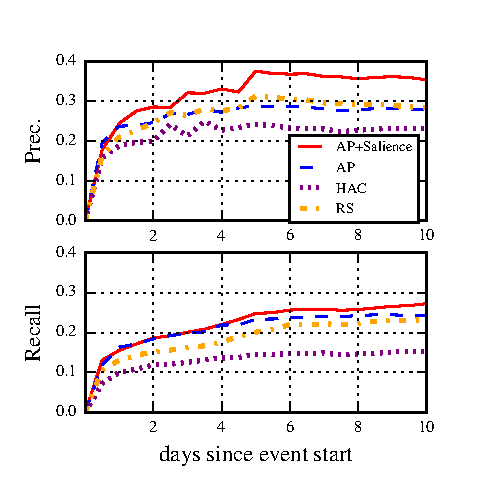
\includegraphics[]{chapter3/figures/rouge-time.eps}
\caption{System ROUGE-1 performance over time.}
\label{fig:3_aps_rouge_time}
\end{wrapfigure}


    \subsubsection{Results}

\autoref{tab:aps_rouge}  shows  our  results  for  system  output
samples against the full summary of nuggets using \textsc{Rouge}. 
This improvement is statistically significant  for  all  ngram  
precision,  recall,  and  F-measures at the
$\alpha=.01$
level using the Wilcoxon
signed-rank test.
\textsc{AP+Salience}
maintains    its    performance
above  the  baselines  over  time  as  well.
\autoref{fig:3_aps_rouge_time}  shows  the  \textsc{Rouge-1}  scores  over  
time.
We  show  the  difference  in  unigram  precision
(bigram  precision  is  not  shown  but  it  follows a
similar  curve).
Within  the  initial  days  of  the
event,  \textsc{AP+Salience}
is  able  to  take  the  lead
over  the  over  systems  in  ngram  precision.   The
\textsc{AP+Salience}
model is better able to find salient
updates earlier on; for the disaster domain, this is
an especially important quality of the model.
Moreover, the \textsc{AP+Salience} recall is not diminished by the high 
precision and remains competitive with \textsc{AP}. 
Over time \textsc{AP+Salience}'s recall also begins to pull away, 
while the other models start to suffer from topic drift.


\autoref{fig:3_aps_autots} shows the Expected Gain and Comprehensiveness 
across a range
of  similarity  thresholds,  where  thresholds  closer
o 1 are more conservative estimates. The ranking
of the systems remains constant across the sweep
with \textsc{AP+Salience}
beating all baseline systems.
Predicting salience in general is helpful for keeping a summary on topic as the  \textsc{RS}  approach out
performs  the  clustering  only  approaches  on  expected gain.
When looking at the comprehensiveness of the
summaries \textsc{AP} outperforms \textsc{AP+Salience}.  
The compromise  encoded  in  the  \textsc{AP+Salience}
objective function, between being representative and
being salient, is seen clearly here where the per-
formance of the \textsc{AP+Salience}
methods is lower
bounded by the salience focused  RS  system and
upper bounded by the clustering only AP system.
Overall, \textsc{AP+Salience}
achieves the best balance
of these two metrics.

\begin{wrapfigure}{R}{0.45\textwidth}
    \center
  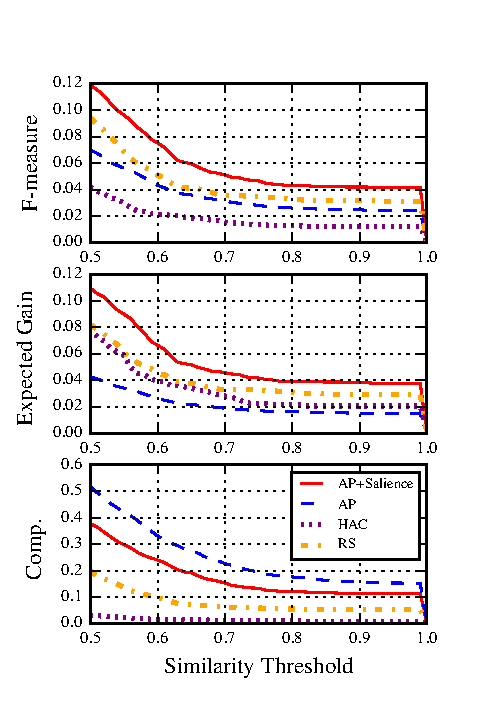
\includegraphics[]{chapter3/figures/nuggets-metrics2.eps}
\caption{Expected Gain and Comprehensiveness performance.}
\label{fig:3_aps_autots}
\end{wrapfigure}



    \subsection{Model 2: LOLS}

Our next model attempts to address some of the shortcomings of the 
first. First the previous model process sentences in hourly batches.
Ideally we would process new documents as soon as possible in order 
to minimize the negative effects of latency. Second, our salience
regressors were statically trained and did not take advantage of features
like the similarity to recently selected updates and relied mostly on
tuned thresholds to account for redundancy. 

Getting around these limitations poses some severe challenges. Using
dynamic features means that naive traing will require gold reference
sentence extracts and that naively training a sentence salience model
with these will under explore the space of plausable update summaries,
meaning that in practice errors are likely to snowball over time.

Instead, we develop a clairvoyant oracle summarizer $\pi^o$ whose behavior
we want to imitate. $\pi^o$ has knowledge of what nuggets, if any, 
are present in each sentence in the document stream, and it's behavior
is quite simple: it processes each sentence in a query's relevant document 
stream and 
when it encounters a sentence with a novel nugget, it adds that sentence
to the update summary.

As we stated before, training only on a single oracle run over document stream
would be sub-optimal because the oracle is perfect and it would finish 
recovering all of the nuggets quite quickly and then do nothing for
the remainder of the stream. In practice, our learned model is likely to
make mistakes, missing the first few appearances of a nugget but hopefully
recovering them as repetition in the stream makes them more likely to be 
selected. Only following the oracle's first best pass would not help us learn
to recover from errors.

To make better use of the oracle, we adopt the locally optimal learning to
search (LOLS) algorithm \cite{lols}, one of a family of learning to search 
(L2S) algorithms. In order to formally describe the algorithm, we first 
introduce some notation. We treat the streaming summarization problem
as a markov decision process. At each timestep $t$ we observe a state
$s_t \in \mathcal{S}$ and $t$-th sentence $x_t \in \mathcal{X}$ from the 
document stream.
A policy $\pi : \mathcal{S} \times \mathcal{X} \rightarrow \{0, 1\}$
maps a state-sentence tuple to an action $a \in \mathcal{A} =\{0,1\}$
where $a=1$ indicates we extract the sentence and $a=0$ indicates we skip
the current sentence. The transition function 
$d : \mathcal{S} \times \mathcal{X} \times \mathcal{A} \rightarrow \mathcal{S}$
deterministically maps state-sentence-action tuples to the next state. 
In practice the state contains set of sentences previously extracted and
other rolling statistics from previously observed sentences in the stream.
Our training objective is to minimize the expected costs of each action:
\[ \mathcal{L}(\pi) = \mathbb{E}_{s,x \sim \pi} \left[ c\left(\pi(s,x), s, x\right) \right] \]
where $c :\mathcal{A} \times \mathcal{S} \times \mathcal{X} \rightarrow \mathcal{A}$ is the cost of taking a given action in a particular state-sentence
observation.

~\\

~\\

In the LOLS training regime, there are two phases: the 
\emph{roll-in} and the \emph{roll-out}. The roll-in phase 

at each timestep 
we alternate between using the oracle $pi^o$ or our current learned policy
$\hat{\pi}$ to run multiple time steps into the future and get a cost for 
a hypothetical summary we would have created in the case where we extracted the 
current sentence or skipped it. We collect these scores for each decision
and update a regression model to accuractely predict the cost of each action
given the current sentence and update summary/stream state.





\subsubsection{Data}
We ran 

\subsubsection{Oracle Policy and Loss Function}

We use a greedy oracle that selects sentences that contain novel
nuggets. This oracle will achieve an optimal Comprehensiveness score, i.e.
it will obtain every possible novel nugget in the roll-out phase.
However, it will not always achieve the maximum possible Expected Gain.
For example, consider the sequence of sentences $s_1, s_2, s_3$, where
nugget $n_1 \in s_1$, $n_2 \in s_2$, and $n_1,n_2 \in s_3$. The greedy oracle,
proceeding sequentially would select sentences $s_1$ and $s_2$, and skip
$s_3$, achieving an Expected Gain of $\frac{|\{n_1, n_2\}|}{|\{s_1, s_2 \}|} = \frac{2}{2} = 1$. The maximum achievable Expected Gain is obtained by skipping
the first two sentences and selecting sentence $s_3$ yielding $\frac{|\{n_1, n_2\}|}{|\{s_3 \}|} = \frac{2}{1} = 2$. In practice we are far from matching
the greedy oracle and so it suffices for now as an aspirational target.



We used the complement of Dice coefficient as the loss function.



\subsubsection{Experiments }

In our results, we refer to our learn-to-search approach as LS.
We compare to a lead sentence baseline that takes the first sentence
of every document as an update if it's maximum cosine similarity to any 
previous update was below a threshold. We refer to this method as COS.

We also compare our 








suboptimal in that it will achieve a perfect
Comprehensiveness 



}{}





\section{Deep Learning Models of Word and Sentence Salience}

\label{sec:chapter4}

\def\tfidf{TF-IDF}

Estimating the salience of words and phrases is core to the problem of 
summarization. For example, \cite{luhn1958automatic} 
noted how the most topically central words in a document occur not too much 
but not
too little, and that,
``the presence in the region of highest frequency of many of the words
 previously described as too common to have the  type  of
 significance being sought would constitute
`noise' in the system.''

Subsequently, many methods have been proposed for salience estimation
in the context of summarization. Word weights have typically been derived
in an unsupervised way from a large collection of in-domain text.
The classic example here is Term Frequency-Inverse Document Frequency
(\tfidf) weighting \citep{sparck1972statistical}, whose aim is similar in 
spirit to Luhn's: important 
words occur frequently in the current context (the term frequency component)
 but not so much that they occur in every document 
(the inverse frequency component).

While \tfidf weights (and others like BM25 \citep{bm25}) have been frequent
ingredients in many summarization systems \citep{a,b,c,d,e}, they are 
not specifically tuned to any one summarization task. Another prominent
strand of research has been the learning of word or ngram specific weights
typically for use in linear models of salience \citep{martins2009summarization,woodsend2010automatic,berg2011jointly,durrett2016learning}. 
Given the small size of most summarization datasets at the time, one could question 
the utility of learning ngram weights when it was unlikely that there 
would be adequate data to learn broad coverage summarizers.

This 
situation has changed with the recent availability of large scale summarization data \citep{cnndm,newsroom,nyt}. With these corpora,
and other developments in word embedding representation \citep{miklov,glove},
many researchers have been developing end-to-end models of both 
abstractive \citep{abs} and extractive \citep{ext} summarization.
While the spirit of ``let a thousand architectures bloom'' has spurred much
creativity and performance gains, it has left us with little explainability
about how such models work. 

While different components of the neural architectures may be justified 
by intuition, these methods are largely black boxes and it is not clear
how they are making their sentence selection predictions. This is especially
problematic in abstractive summarization, but it is also not well understood
how extractive methods make their decisions either.

In this chapter, we describe completed experiments teasing out the importance
of different neural network designs for sentence level salience. This
work describes impedements to learning and word and sentence representations
in deep learning models of extractive summarization, and led to 
a recent publication \citep{kedzie2018deep}. Based on these limitations,
we propose extensions to the word level representations and explicitly model
word level salience scores as a means to performing sentence extractive
summarization. While the finished and proposed work focuses on single document
summarization, we also propose an extension of the word level salience
estimation model that we hope will generalize to the multi-document
summarization context.


%In this chapter we investigate neural network architectures for extractive
%summarization, in the hopes of better understanding what is important 
%for the underlying word and sentence representations to learn.
%We start a description of completed experiments for sentence extractive
%models of summarization \citep{kedzie2018deep}, and then complete the chapter with a description
%of planned and ongoing word importance estimation techniques using deep
%learning models.


~~\\
~\\






Increasingly, researchers are returning to single document summarization,
once thought to be too difficult for automatic summarization methods.
This has been driven both by the availability of large corpora (the
most popular corpus, CNN-DailyMail, has a little over 300,000 data points
\citep{see2017get}) and by the development of general purpose 
generative models of text from the neural machine translation community.
Accordingly, the bulk of the research has used this corpus, (and the NYT
corpus \citep{sandhaus2008new}) to focus on abstractive summarization
research \citep{rush2015neural,chopra2016abstractive,cheng2016neural,nallapati2016abstractive,see2017get,paulus2017deep}. 
There has been a smaller but similar proliferation of sentence
extractive single document summarization papers on these corpora also using 
neural network architectures \citep{cheng2016neural,nallapati2016classify,nallapati2016abstractive,narayan2018ranking}.



\ifthenelse{\equal{\highlevel}{false}}{
  
\newcommand{\sent}{s}
\newcommand{\Sents}{\mathcal{S}}
\newcommand{\doc}{D}
\newcommand{\lbl}{y}
\newcommand{\Labels}{Y}
\newcommand{\word}{w}
\newcommand{\vocab}{\mathcal{V}}
\newcommand{\extracts}{\mathcal{E}}
\newcommand{\budget}{c}
\newcommand{\encoder}{\textsc{Encoder}}
\newcommand{\extractor}{\textsc{Extractor}}
\newcommand{\embproj}{W}
\newcommand{\emb}{\omega}
\newcommand{\embsize}{n}
\newcommand{\sembsize}{m}
\newcommand{\semb}{h}
\newcommand{\rsemb}{\overrightarrow{\semb}}
\newcommand{\lsemb}{\overleftarrow{\semb}}
\newcommand{\gru}{\textsc{Gru}}
\newcommand{\rgru}{\overrightarrow{\gru}}
\newcommand{\lgru}{\overleftarrow{\gru}}
\newcommand{\cfeat}[2]{f_{#1}^{( #2 )}}
\newcommand{\relu}{\textsc{ReLU}}
\newcommand{\winsize}{k}
\newcommand{\winsizes}{K}
\newcommand{\fmapsize}{F}
\newcommand{\cfidx}{l}
\newcommand{\cact}{a^{(\cfidx,\winsize)}}
\newcommand{\cnnbias}{u^{(\winsize)}}
\newcommand{\cnnweight}{U^{(\winsize)}}
\newcommand{\cnnBiasSpace}{\mathbb{R}^{\fmapsize_\winsize}}
\newcommand{\cnnWeightSpace}{\mathbb{R}^{\winsize \times \fmapsize_\winsize \times \embsize}}


\subsection{Deep Learning Models of Sentence Extraction}

 Given the diversity of neural architectural choices, a best practices
for sentence extracive summarization has yet to emerge. In this section
we ask what architecture design choices matter for single document 
summarization across a variety of domains.

We begin by definining some terminology. A sentence is represented as an
sequence of words $\sent = \{\word_1, \word_2, \ldots, \word_{|\sent|} \}$
where each word is drawn from a fixed vocabulary $\vocab$ and $|\sent|$ is
the length of sentence $\sent$ in words. Similarly, a document $\doc = \{ 
\sent_1, \sent_2, \ldots, \sent_{|\doc|} \}$ is a sequence of sentences, where 
$|\doc|$ is the size of the document in sentences.  

We treat the sentence extractive summarization as sequence tagging
problem: given a document $\doc$, we want to assign an associated binary
tag sequence $\Labels = \{\lbl_1, \lbl_2, \ldots, \lbl_d \}
\in \{0,1\}^d$ such that the extract summary $\extracts = \{ 
\sent_i \in \doc : \lbl_i =1 \}$ implied by $\Labels$ is a suitable summary
of the document. Typically, it is assumed that size of the extract summary
$|\extracts| = \sum_{i=1}^{|\doc|} \mathbbm{1}\{\lbl_i =1 \} \ll |\doc|$.
It is also common to enforce a word budget $\budget$ such that
$\sum_{\sent \in \extracts} |\sent| \le \budget$.

A typical deep learning model will build up a hierarchical representation
of each sentence, starting at the word level, and then composing an arbitrarily
long sequence of word representations into a fixed length sentence 
representation.
First the individual words are 
projected to fixed length vectors, or word embeddings via a mapping
$\embproj : \vocab
\rightarrow \mathbb{R}^{\embsize}$. The sentence encoder network $\encoder :
\{\mathbb{R}^{\embsize}\}^* \rightarrow \mathbb{R}^{\sembsize}$ is then 
responsible for mapping word embbeding sequences to fixed length sentence 
embeddings. Finally, the sentence extractor network $\extractor : 
\{\mathbb{R}^\sembsize\}^* \rightarrow \{0, 1\}^*$ produces a label 
sequence $\Labels$.

We explore several choices of encoder and extractor architecture from the 
literature \citep{cheng2016neural,nallapati2016summarunner} as well as 
propose our own designs \citep{kedzie2018deep}. In the next sections,
we describe the three sentence encoder architectures (\textit{avg}, 
\textit{rnn}, and \textit{cnn}) followed by four extractor architectures 
(\textit{rnn}, \textit{seq2seq}, \textit{sr}, and \textit{cl}).

\subsubsection{Sentence Encoders}
\paragraph{Averaging} The simplest encoder simply averages a sentence's
associated word embeddings:
\[ \encoder_{avg}(\sent) = \frac{1}{|\sent|} \sum_{\word \in \sent} \embproj(\word). \]
Other than the word embeddings, this encoder involves no learned parameters,
and while it collapses word order, embedding averaging has consistently
been found competitive with more sophisticated sentence embedding techniques
\citep{iyyer2015deep,wieting2015towards,arora2016simple,wieting2017revisiting}.


\paragraph{Recurrent Neural Networks} The second encoder architecture
we experiment with is a recurrent neural network (RNN) over the word
embeddings. An RNN maintains an internal ``hidden'' state that is sequentially
updated upon observing each word embedding. In practice, we use a bidirectional
RNN with a gated recurrent unit (GRU) as the particular instantiation of 
the RNN cell \citep{cho2014learning}.
Under the RNN encoder, a sentence embedding for a sentence $\sent$ is defined 
as
\begin{align}
\encoder_{rnn}(\sent) = [\overrightarrow{\semb}_{|\sent|}, \overleftarrow{\semb}_{1} ] & \\
  \rsemb_0 = \mathbf{0};& \quad 
  \rsemb_i = \rgru\left(\embproj(\word_i), \rsemb_{i-1}\right) \\
  \lsemb_{|\sent| + 1} = \mathbf{0};& \quad 
  \lsemb_i = \lgru\left(\embproj(\word_i), \lsemb_{i+1}\right) 
\end{align}
where $[\cdot]$ is the concatenation operator; $\rsemb_i$ and $\lsemb_i$ are
hidden states of the forward and backward GRU cells respectively; and 
$\rgru, \lgru : \mathbb{R}^\embsize \times \mathbb{R}^\sembsize 
\rightarrow \mathbb{R}^\sembsize$ are the forward and backward GRU cell 
operations.
\cite{nallapati2016summarunner} use a bidirectional RNN for their sentence
encoder.

\paragraph{Convolutional Neural Networks}
Our final sentence encoder uses a convolutional neural network
(CNN) to encode important ngram windows into a fixed length vector. 
CNN's have grown increasingly popular in many NLP tasks 
as a computationally efficient substitute for RNN-based architectures
\citep{kim2014convolutional,lei2015molding,dauphin2017language}.
Our architecture largely follows \cite{kim2014convolutional}: we apply a 
series of one dimensional convoluions over a sentence's word embeddings
using varying width convolutions. For each convolutional window size 
$\winsize \in \winsizes \subset \mathbb{N}$, a convolutional filter creates 
a feature vector $\cfeat{}{\winsize} \in \mathbb{R}^{\fmapsize_\winsize}$ 
and the encoder output is the concatenation of the $|\winsizes|$ vectors. 
The set of filter window sizes $\winsizes$ and the number of feature maps
$\fmapsize_\winsize$ for each $\winsize \in \winsizes$ are 
model hyperparameters.
Formally, we define the CNN encoding of a sentence $\sent$ as 
\begin{align}
\encoder_{cnn}(\sent) & = \left[\cfeat{}{\winsize} : \winsize \in \winsizes \right]\\
\cfeat{\cfidx}{\winsize} &= 
     \max_{i \in 1,\dots, |\sent| - \winsize + 1} 
       \relu\left(\cact_i \right) \\
\cact_i &= \cnnbias_\cfidx
    + \sum^{\winsize}_{j=1} \cnnweight_{\cfidx,j} \cdot \embproj(\word_{i + j -1})
\end{align}
where $\cnnbias \in \cnnBiasSpace$ and $\cnnweight \in \cnnWeightSpace$
are learned convolutional filter weights and $\relu(x) = \max(0, x)$ 
is the rectified linear unit \citep{nair2010rectified}. \cite{cheng2016neural}
uses a CNN for their sentence encoder.

\subsubsection{Sentence Extractors}

A sentence extractor takes the encoder output, i.e. 
a sequence of sentence embeddings
$\encoder(\doc) =$ $\{\encoder(\sent_1), \ldots, \encoder(\sent_{|\doc|})\} =
\{\semb_1, \ldots, \semb_{|\doc|}\}$, and produces a sequence of labels
$\Labels = \{\lbl_1, \ldots, \lbl_{|\doc|}\}$. 
The sentence extractor is essentially a discriminative
classifier $p(\lbl_1,\ldots,\lbl_{|\doc|} | \semb_1,\ldots,\semb_{|\doc|})$.
Previous neural network approaches to sentence extraction have assumed
an auto-regressive model, leading to a semi-Markovian
factorization of the extractor probabilities
$p(\lbl_{1:n}|\semb)=\prod_{i=1}^{|\doc|} 
p(\lbl_i|\lbl_{<i},\semb)$,
where each prediction $\lbl_i$ is dependent on \emph{all}
previous $\lbl_j$ for
all $j < i$. We compare two such models proposed by \cite{cheng2016neural}
and \cite{nallapati2017summarunner}.
A simpler approach that does not allow interaction among the $\lbl_{1:n}$
is to
%\hal{a simpler approach (explain why simpler) is a fully factored representation 
  model $p(\lbl_{1:n}|\semb) = \prod_{i=1}^n p(y_i|h)$,
  which we explore in two proposed extractor models that we refer to as the RNN 
  and Seq2Seq extractors.
%Implementation details for all extractors are in \autoref{app:sentextractors}.


%\paragraph{Previously Proposed Sentence Extractors}
% We consider two recent state-of-the-art extractors.
\paragraph{Cheng \& Lapata Extractor} 
 The first extractor we consider, proposed by 
\citet{cheng2016neural}, %, which we refer to as the Cheng \& Lapata Extractor,
is built around a sequence-to-sequence model.
First, each sentence embedding\footnote{\citet{cheng2016neural} used an CNN sentence encoder with 
this extractor architecture; in this work we pair the Cheng \& Lapata extractor
with several different encoders.} is
fed into an encoder side RNN, with the final encoder state passed to the
first step of the decoder RNN. On the decoder side, the same sentence 
embeddings are fed as input to the decoder and decoder outputs are used to
predict each $\lbl_i$. The decoder input is weighted by the previous extraction
probability, inducing the dependence of $\lbl_i$ on $\lbl_{<i}$.
See \autoref{fig:extractors}.c for a graphical layout of the extractor.
%and \autoref{app:clextractor} for details.

%?, but are delayed by one step and 
%?weighted by their prediction probability, i.e. at decoder step $t$,
%?$p(\slabel[t-1]|\slabel[<t-1], \sentEmb[<t-1]) \cdot \sentEmb[t-1]$\hal{why did you switch from $i$ to $t$?}
%?is fed into the decoder\hal{i don't udnerstand what this means. what op is $\cdot$?}. The decoder output at step $t$ is concatenated 
%?to the encoder output step $t$ and fed through a multi-layer perceptron
%?with one hidden layer and sigmoid unit output computing the $t$-th
%?extraction probability $p(\slabel[t]|\slabel[<t], \sentEmb[<t])$. \textcolor{red}{See Figure 2.c. for a graphical view. Full model details are presented in ??}.
%?

\paragraph{SummaRunner Extractor}\citet{nallapati2017summarunner} proposed
a sentence extractor, which we refer to as the SummaRunner Extractor,
that factorizes the extraction probability into contributions 
from different sources.
First, a bidirectional RNN is run over the sentence embeddings\footnote{\citet{nallapati2017summarunner}
    use an RNN sentence encoder with 
this extractor architecture; in this work we pair the SummaRunner extractor
with different encoders. } and the output is
concatenated. A representation of the whole document is made by 
averaging the RNN output. A summary representation is also constructed 
by taking the sum of the previous RNN outputs weighted by their extraction
probabilities. Extraction predictions are made using 
the RNN output at the $i$-th step, the document representation, and 
$i$-th version of the summary representation, along with factors for 
sentence location in the document. The use of the iteratively constructed
summary representation creates a dependence of $\lbl_i$ on all $\lbl_{<i}$.
See \autoref{fig:extractors}.d for a graphical layout.
%

%\paragraph{Proposed Sentence Extractors}
%We propose two sentence extractor models that 
%make a stronger conditional independence 
%assumption $p(\slabel|\sentEmb)=\prod_{i=1}^\docSize p(\slabel[i]|\sentEmb)$,
%essentially making independent predictions conditioned on $\sentEmb$.


\paragraph{$\extractor_{rnn}$}
    Our first proposed model is a very simple bidirectional
RNN based tagging model. As in the RNN sentence encoder we use a GRU cell.
The forward and backward outputs of each sentence are passed through a 
multi-layer perceptron with a logsitic sigmoid output 
to predict the probability
of extracting each sentence. 
See \autoref{fig:extractors}.a for a graphical layout.
%and \autoref{app:rnnextractor} for details.


\newcommand{\rExtHidden}{\overrightarrow{h}}
\newcommand{\lExtHidden}{\overrightarrow{h}}
\newcommand{\docSize}{|\doc|}
\newcommand{\logits}{o}

\begin{align}
    \rExtHidden_0 = \mathbf{0};&\quad   \rExtHidden_i = \rgru(\semb_i, \rExtHidden_{i-1}) \\
    \lExtHidden_{\docSize + 1} = \mathbf{0};&\quad    \lExtHidden_i = \lgru(\semb_i, \lExtHidden_{i+1}) \\
   \logits_i &= \relu\left(U \cdot [\rExtHidden_i; \lExtHidden_i] + u \right)\\
    p(\lbl_i=1|\encoder(\doc)) &= \sigma\left(V\cdot \logits_i + v  \right)
\end{align}
where $\rgru$ and $\lgru$ indicate the 
forward and backward GRUs respectively, and each have separate learned 
parameters; $U, V$ and $u, v$ are learned weight and bias parameters.
The hidden layer size of the GRU is 300 for each direction and the MLP hidden layer
size is 100. Dropout is applied to the GRUs and to $a_i$.





\paragraph{$\extractor_{s2s}$} One shortcoming of the RNN extractor is that long range
information from one end of the document may not easily be able to affect 
extraction probabilities of sentences at the other end. 
Our second proposed model, the $\extractor_{s2s}$ mitigates this problem with an 
attention 
mechanism commonly
used for neural machine translation \cite{bahdanau2014neural} and 
abstractive summarization \cite{see2017get}. 
The sentence embeddings are first
encoded by a bidirectional $\gru$. A separate decoder $\gru$ transforms each 
sentence into a query vector which attends to the encoder output. The
attention weighted encoder output and the decoder $\gru$ output are concatenated
and fed into a multi-layer perceptron to compute the extraction probability.
See \autoref{fig:extractors}.b for a graphical layout.




\subsection{Experiments}

 We are interested in two questions. The first, more pragmatic question, is
 what are the best configuration of encoder/extractor architectures?
 We answer this question by evaluating ROUGE recall and METEOR \citep{meteor}
 performance across our six collected datasets. We perform the standard
 stochastic gradient descent \cite{sgd} based optimization (using the Adam
 update \cite{adam}) of the weighted negative log likehood 
 \[ \mathcal{L}(\theta) = -\sum_{\Sents, \Labels \in \mathcal{D}} 
            \sum_i \omega(\lbl_i) 
        \log p(\lbl_i|\lbl_{<i}, \Sents; \theta) \]
        where $\theta$ are model parameters and $\omega(\lbl_i)$ upweights
        the positive labels to account for the imbalanced label distribution.

 We lack human reference extract labels for our datasets and so we obtain
 said lable sequences heuristically, by finding a label sequence $\Labels^*$
 by greedily optimizing ROUGE-1 recall with respect to the human reference
 abstracts.

 The second question, is more diagnostic in nature: what signals
 in the data are driving model learning?
 We perform several experiments to find answers. 
 We hypothesize that the lexical semantics encoded at the word embedding
 level will be important to subsequent sentence representations, and
 perform a comparison on learning with and with out fine tuning of the 
 embeddings. In both cases, embeddings are initialized with Glove
 embeddings pretrained on Wikipedia and Gigaword \citep{glove}.
 
 
 We also hypothesize that certain classes of words will be more important 
 to identifying salient content than others. We perform word ablation 
 experiments where we alternately remove nouns, verbs, adjectives \& adverbs,
 and function words from the sentence encoder input and compare performance 
 to the non-ablated system. We expect that the nouns will be more important
 to content selection. 


 Our final experiments attempt to tease out the effect of structural features 
 from the lexical. In this experiment, we shuffle the sentence order at 
 training time. In this setup, we obfuscate features about which content 
 was introduced in the article first, an important and well known bias in 
 news domain \cite{leadbias}. 


 \subsection{Results}


  

The results of our main experiment comparing 
the different extractors/encoders are shown in 
Table~\ref{tab:results}.
Overall, we find no major advantage when using the CNN and RNN sentence
encoders over the averaging encoder. The best performing encoder/extractor pair either 
uses the averaging 
encoder (five out of six datasets) or the differences 
are not statistically significant. %When only comparing within the 
%same extractor choice,  the averaging encoder is the better choice
%in 14 of 20 cases. 
%\hal{i wonder if it would be worth adding another ``average performance metric'' column to \autoref{tab:results}.
%  i'm thinking have ``Average $\Delta$-Best'' meaning how far (on average across the datasets) is this setting from the best setting available on that dataset.
%  so since the best numbers are: 25.56, 35.85, 23.11, 13.65, 5.63
%  and the first row numbers are: 25.42, 34.67, 22.65, 11.37, 5.50
%  then the deltas are:            0.14,  1.18,  0.46,  2.28, 0.13
%  the the average delta is 0.84 (assuming my math is right)
%  there's an argument to do multiplicative, in which case
%  the multipliers for first row:  0.99,  0.97,  0.98,  0.83, 0.97
%  and the average is 0.95
%  either way this gives a quick way to make comparisons between rows. you could do the same for the other tables too.}

  %\hal{in some of the tables you list R-2 as headers even though all the numbers are R-2. just put that in the caption.}


When looking at extractors, the Seq2Seq extractor is either part of 
the best performing system (three out of six datasets) or is not 
statistically distinguishable from the best extractor. 

Overall, on the news and medical journal domains, the differences are 
quite small with the 
differences between worst and best systems on the CNN/DM dataset 
spanning only .56 of a ROUGE point. While there is more performance variability
 in the Reddit and AMI data, there is less distinction among systems: 
 no differences are significant on Reddit
and every extractor has at least one configuration that is indistinguishable
from the best system on the AMI corpus. This is probably due to the small test
size of these datasets.
%\hal{this is probably at least partially because of test set size. maybe mention this.}





%?\textcolor{red}{Overall we find that the \modelTwoBF~extractor achieves the 
%?best ROUGE scores on three out of four domains (STILL RUNNING ON AMI AND PUBMED). 
%?However, most
%?differences are not signficant. (Need to discuss stat sig and how to show it).}
%?On the larger CNN-DailyMail dataset, especially, 
%?differences are quite smail across all extractor/encoder pairs.
%?The \baselineOneBF~extractor achieves the best performance on the DUC 2002
%?dataset. It is disappointing that the \baselineOneBF~and \baselineTwoBF~based 
%?models do not gain any apparent advantage in conditioning on previous 
%?sentence selection decisions; this result suggests the need to improve
%?the representation of the summary as it is being constructed iteratively.
%?
%?\textbf{Choice of Encoder} We also find there to be no major advantage 
%?between the different sentence encoders. \textcolor{red}{In most cases,
%?there is no statistical significance between the averaging encoder and either
%?the RNN or CNN encoders.} 

%The lack of differentiation amongst the different encoders concerning; one
%would assume learning with the appropriate structure would be helpful.
%The results of next 




\paragraph{Word Embedding Learning}
 Given that learning a sentence encoder (averaging has no learned parameters)
 does not yield significant improvement, it is natural to consider whether
 learning word embeddings is also necessary. 
 In \autoref{tab:embeddings} we compare the performance of different extractors
 using the averaging encoder, when the word embeddings are held fixed or 
 learned during training. In both cases, word embeddings are initialized with
 GloVe embeddings trained on a combination of Gigaword and Wikipedia.
% \hal{TRAINED ON WHAT? JUST THE DEFAULT ONES?}
 When learning embeddings, words occurring 
 fewer than three times in the training data are mapped to an unknown
 token (with learned embedding).
 
% shows ROUGE recall
%when using fixed or updated word embeddings. 
 In all but one case,
fixed embeddings are as good or better than the learned embeddings.
This is a somewhat surprising finding on the CNN/DM data since it is reasonably
large, and learning embeddings should give the models more
flexibility to identify important word features.\footnote{The AMI corpus is an exception here where learning \emph{does} lead to small
performance boosts, however, only in the Seq2Seq extractor is this diference 
significant; it is quite possible that this is an artifact of the very small
test set size.}
%\hal{why is it surprising?} \textcolor{green}{[[CK: Because learning embeddings should give the model more capacity to represent important patterns]]}
This suggests that we cannot extract much generalizable learning signal 
from the content other than what is already present from initialization. 
Even on PubMed, where the language is quite different from the news/Wikipedia
articles the GloVe embeddings were trained on, learning leads to 
significantly worse results.

%The language of this corpus is quite different from the 
%data that the GloVe embeddings were trained on and so it makes sense 
%that  there would be more benefit to learning word representations; one
%explanation for only seeing modest improvements is purely the small size
%of the test dataset which has only 20 training meetings.

%textcolor{red}{(NOTE TO CK -- expect learning to help on pubmed)}. \hal{yes, the dataset size is certainly an issue here. probably worth pointing this out. also when you learned the embeddings, did you initialize to pretrained embeddings? did you regularize toward them?}


\paragraph{POS Tag Ablation}
It is also not well explored what word features are being used by the encoders.
To understand which classes of words were most important we ran an ablation
study, selectively removing nouns, verbs 
(including participles and auxiliaries), adjectives \& adverbs, and 
function words (adpositions, determiners, conjunctions).
%Additionally, we ran ablation experiments
%using part-of-speech (POS) tags. \hal{this needs to be justified. why is this experiment interesting?}
All datasets were automatically tagged using
the spaCy part-of-speech (POS)
tagger\footnote{https://github.com/explosion/spaCy}.   
%\kathy{I'm still curious what would happen if you separately removed all conjunction tags and later remaining POS.}
%We experimented with selectively removing 
%\begin{itemize}
%    \item nouns (NOUN and PROPN tags), 
%    \item verbs (VERB, PART, and AUX tags), 
%    \item adjectives/adverbs (ADJ and ADV tags), 
%    \item numerical expressions (NUM and SYM tags), and 
%    \item miscellaneous words (ADP, CONJ, CCONJ, DET, INTJ, and SCONJ tags)
%\end{itemize}
%from each sentece. 
The embeddings of removed words were replaced with a zero vector,
preserving the order and position of the non-ablated words in the sentence.
Ablations were performed on training, validation, and test partitions,
using the RNN extractor with averaging encoder.
\autoref{tab:ablations} shows the results of the POS
tag ablation experiments. 
While removing any word class from the representation generally hurts 
performance (with statistical significance), on the news domains,
the absolute values of the differences are quite small 
(.18 on CNN/DM, .41 on NYT, .3 on DUC) suggesting that the model's predictions
are not overly dependent on any particular word types.
On the non-news datasets, the ablations have a larger effect 
(max differences are 1.89 on Reddit, 2.56 on AMI, and 1.3 on PubMed).
Removing nouns leads to the largest drop on AMI and PubMed.
Removing adjectives and adverbs leads to the largest drop on Reddit,
suggesting the intensifiers and descriptive words are useful for 
identifying important content in personal narratives.
Curiously, 
removing the function word POS class yields a significant improvement
on DUC 2002 and AMI.


%The newswire domain does not appear to be sensative
%to these ablations; this suggests that the models are still able to identify
%the lead section of the document with the remaining word classes \textcolor{red}{(Verify this with histogram analysis)}. 
%The Reddit domain, which is not lead biased, is significantly effected.
%Notably, removing adjectives and adverbs results in a 1.8 point drop 
%in ROUGE-2 recall. 


\textbf{Document Shuffling} Sentence position is a well known and 
powerful feature for news summarization \cite{hong2014improving}, owing 
to the intentional lead bias in the news article writing\footnote{\url{https://en.wikipedia.org/wiki/Inverted_pyramid_(journalism)}}; it also explains the difficulty in beating
the lead baseline for single-document summarization 
\cite{nenkova2005automatic,rau:1999}.
In examining the generated summaries, we found
most of the selected sentences in the news domain came from the lead paragraph
%\hal{i feel like there must be citations to dig up here from like the 90s about lead summarization in news... it's also an intentional bias: maybe the right thing is to cite a style guide from a newsppaer that says to write this way}
of the document. This is despite the fact that there is a long tail of 
sentence extractions from later in the document in the ground truth extract 
summaries (31\%, 28.3\%, and 11.4\% of DUC, CNN/DM, and NYT training extract labels come 
from the second half of the document). 
%\hal{can you be more specific? like give some stats? what \%age come from first quarter of doc and what \%age from last half or something}. 
Because this lead bias is so strong, it is questionable whether
the models are learning to identify important content or just find the start
of the document. We conduct a sentence order experiment where 
each document's sentences are randomly shuffled during training. We then
%KM - I think below should be shuffled. I changed.
%CK - models are trained on shuffled data but evaluated on in order models.
%evaluate each model performance on the unshuffled test data, comparing to 
evaluate each model performance on the unshuffled test data, comparing to 
the model trained on unshuffled data; if the models trained on shuffled data
drop in performance, then this indicates the lead bias is the relevant factor.
%in learning content selection.

\autoref{tab:shuffle} shows the results
of the shuffling experiments. 
The news domains and PubMed suffer a significant drop in performance 
when the document order is shuffled. By comparison, there is no significant difference between the shuffled and in-order models on 
the Reddit domain, and shuffling actually improves performance on AMI.
%\hal{what about in the cross-domain setting?} 
This suggest that position 
is being learned by the models in the news/journal article domain even when 
the model has no explicit position features, and that this feature is more 
important than either content or function words.












  \def\word{w}
\def\vocab{\mathcal{V}}
\def\contextFeatures{\textsc{Context}}
\def\wordFeatures{\textsc{Word}}
\def\elmo{\textsc{Elmo} }
\def\wordImportance{z}
\def\aggWordImportance{\eta}
\def\sent{s}
\def\bow{\omega}
\def\labels{y}
\def\predLabels{\hat{\labels}}

  \subsection{Word Importance Estimation in Deep Learning Models}


\begin{figure}
 \begin{center}
  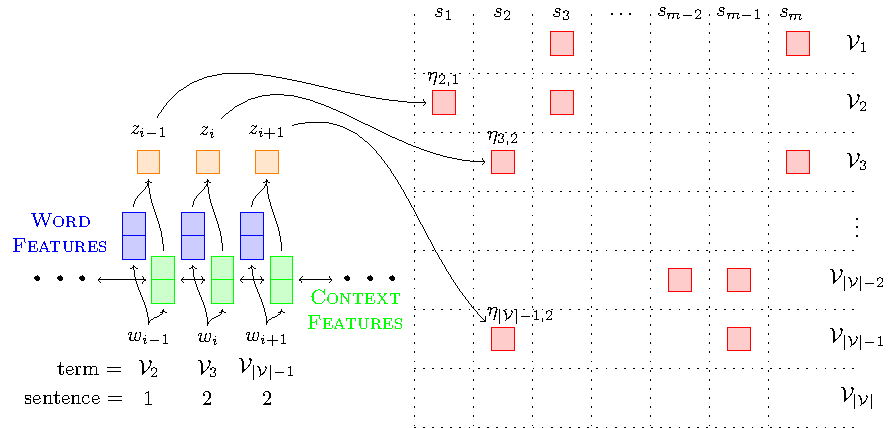
\includegraphics[scale=.7]{chapter4/figures/4_2_wimp_model.pdf}
 \end{center}
\caption{Left: Word and context features are extracted from the flat token
sequence representation to get word level importance scores 
$\wordImportance_i$. Right: word level scores are aggregated into a sparse
bag-of-words representation of the input sentences.}
\end{figure}

Our previous experiments revealed that lexical sematics were not the 
main driver of learning in sentence extractive news summarization. 
One could plausibly argue that it is a feature, not a bug, and that 
the structural
signals in news are intentional and not to be avoided. However, we think more 
attention could be paid to estimating importance scores at the word level.
We are motivated by potential application to abstractive generation: better
word level importance estimation could help to remove all but the most 
necessary content from the documents as a preprocessing stage before
abstractive summarization. We are also encouraged by parallel practices
in multi-lingual news summarization, where word importance weights 
are the main ingredient in sentence representations. 


\newcommand{\mlingsys}{\textsc{Classy}}

%\subsubsection{A brief discussion of \mlingsys.}

\mlingsys and its antecedents have been consistent top performers in various
summarization workshops \cite{tac,multiling}. In general the main approach 
is to represent each sentence as a sparse bag-of-words, where non-zero
entries correspond to word importance weights for the words found in the 
sentence. Typically, tf-idf weights are used for the importance scores.
The term by sentence matrix representing the document or documents to be
summarized is then factorized into two low rank matrices (typically with
non-negative entries) representing term factors and sentence factors.
The entries in the sentence factor matrix represent latent factors, 
and apriori the importance of each sentence is the sum of its latent factors.

Sentence selection can subsequently be performed using one of several methods.
In the naive case, one can select the sentence with the highest vector norm, 
substract the selected latent factors from the remaining sentence vectors
(zeroing out any terms that become negative), and repeating until the
summary length budget is reached. More sophisticated selection procedures
involving multi-dimensional knapsack packing or submodular optimization 
can be used, however these are not the focus of this work.

One draw back to this approach is that the sentence factors and word 
importance scores are unsupervised with respect to the final summarization
objective; their utility to the summarization task is a happy coincidence.
Additionally, the word importance scores are not assigned based on the 
context in which the word appears.

We propose to address these issues by learning word level importance 
scores in the process of single document sentence extractive summarization.
Additionally, we propose a method of adapting these scores from the 
single document case to multi-document summarization.

\subsubsection{Proposed Model}


In our proposed model for word importance, we estimate the importance of
each word in the context it occurs by first running the ELMO model
over all the words in the document to obtain contextual representations
of each word. The ELMO embeddings are then combined with pretrained Glove
embeddings, document frequency embeddings, topic signature embeddings,
sentence position embeddings, and part-of-speech tag embeddings and then
fed into a multi-layer perceptron to predict a scalar importance score.
When a word occurs multiple times in the input, it can be given a different 
importance score at each location because the ELMO embeddings will capture
contributions of the salient neighbor words. A term-sentence matrix is 
then formed from the input, using the estimated word importance scores 
as the term weights. A sentence extractive summary can be obtained 
using the naive sentence selection method described above or in Figure ?.
The total score for the summary can also be obtained.

We can train this summarizer using a gold extract sequence and a margin loss
\[  \max\left(0, 1 + f(\hat{y}) - f(y) \right) \] where $f(\hat{y})$ is
the score of our predicted extract summary.


Let $z_1, z_2, \dots, z_n$ be the bag of words representations of the 
sentences selected for the summary, in the order they were selected.
The score for the summary is computed as 
$\textsc{Score}(z) = \sum_{i=1}^n \sum_{j=1}^k \max(0, z_{i,j} - \sum_{l=1}^{i-1} z_{l,j})$ 


~\\
~\\

Let $\vocab$ be a fixed vocabulary of words. A document is a sequence $m$
words $\word = \{\word_1, \word_2, \ldots, \word_m\} \in \vocab^m$.
We define two mappings of words to dense vector representations.
The first $\fdef{\wordFeatures}{\vocab}{\Rn{d_1}}$ maps words to 
a concatenation of feature embeddings whose total dimension is of size $f$. 
The various components of the feature embeddings include the word's Glove 
embedding, an embedding for sentence position, and other features of the word.
The second mapping
$\fdef{\contextFeatures}{\vocab}{\Rn{d_2}}$ maps the word to it's contextual
embedding; here this corresponds to the output of \elmo at that word's
position in the document. 
The importance score $\wordImportance_i$ of a word $\word_i$ is the output of 
a feedforward layer 
\[ \wordImportance_i = \sigma\Big(W \left[\begin{array}{c} \wordFeatures(\word_i) \\ \contextFeatures(\word_i) \end{array} \right] + b \Big) \]
    where $W \in \Rn{d_1 + d_2}$ and $b \in \R$ are learned weight
and bias parameters, and $\sigma$ is the logistic sigmoid.

Next, we aggregate the flat token level scores into a bag-of-words (BOW) 
representation for each sentence in the document.
Let $I_i$ be the set of indices of the flat word sequence corresponding
to the words in $i$-th input sentence. Let $\bow_i$ be the BOW 
representation of the $i$-th sentence with entries 
\[ \bow_{i,j} = \begin{cases} 
    0 & \textrm{if $\word_k \ne \vocab_j $ for all $k \in I_i $} \\ 
\sum_{k \in I_i} \mathbbm{1}\{\word_k = \vocab_j \} \cdot \wordImportance_k  & \textrm{otherwise}     \end{cases} \]
        for all $j \in \{1, \ldots, |\vocab|\}$.



\begin{figure}
  \begin{algorithmic}[1]
    \Procedure{\textsc{BowExtracter}}{$\bow, \beta, \kappa$}
   
      \State $\bow_i^{(1)}  \gets \bow_i \quad \forall i \in [[n]]$
      \State $\hat{\eta} \gets 0$
      \State $t \gets 0$
      \While{ $\sum_{i=1}^t \kappa_{\predLabels_i} < \beta$ and $t < n$}
        \State $t \gets t + 1$
        \State $\predLabels_t \gets \operatorname{arg max}_{i \in [[n]]}
            \sum_{j=1}^{|\vocab|} \bow^{(t)}_{i,j}$
        \State $\bow_i^{(t+1)} \gets \max(0, \bow_i^{(t)} - \bow^{(t)}_{\predLabels_t} )\quad  \forall i \in [[n]]$
        \State $\hat{\eta} \gets \hat{\eta} + \sum_{j=1}^{|\vocab|} \bow_{\predLabels_t,j}^{(t)}$
         

      \EndWhile
        \State \Return $[\predLabels_1,\ldots,\predLabels_t], \hat{\eta}$ \Comment{Returns summary sentence indices and summary score.}
    \EndProcedure
  \end{algorithmic}
\caption{Simple sentence extraction algorithm given non-negative BOW inputs.}
\label{alg:wimp_ext_alg}
\end{figure}



        With the BOW representations in hand, we perform sentence selection
        using the algorithm presented in \autoref{alg:wimp_ext_alg} to 
        obtain a predicted extract indices $\predLabels$ and their associated
        score $\hat{\eta}$.

        We can optimize this model using a margin loss, where given a 
        gold extract sequence  $\labels$, we can compute the associated
        gold extract summary score $\eta$ and then minimize the following
        loss function \[\mathcal{L}_{ext}(\predLabels, \labels;\theta) = \max\big(0, 1 + \hat{\eta} - \eta\big)\]
        with respect to the parameters of the word importance predictor.
        If needed, we can also introduce a supervised learning signal to the 
        individual word importance scores by collecting labels $\zeta_i$ for
        each $\wordImportance_i$ such that $\zeta_i = 1$ if $\word_i$ occurs
        and any human reference abstract and $0$ otherwise. For the word level
        loss we would use the cross entropy 
        \[ \mathcal{L}_{word}(\wordImportance, \zeta; \theta) = -\sum_{i=1}^m \zeta_i \log \wordImportance_i + (1 - \zeta_i) \log (1 - \wordImportance_i). \] 




        \paragraph{Adaptation to MDS} We also propose a simple 
        self attention-based modification to
        the word importance aggregation step to help adapt this method
        to multi-document summarization (MDS). \citep{conroy} found
        that dimensionality reduction on the BOW representations improves
        summarizer performance in the MDS setting (but not on single document
        summarization). 


        We plan to experiment with the following importance 
        aggregation method. First, given the outputs of the contextual features
        $h_i$, we compute a self attention matrix $\Lambda \in \Rn{m\times m}$
        where \[\Lambda_{i,j} = \sigma(h_i \cdot h_j / \tau + b)  \]
        using sigmoidal attention \cite{strucattn} with a learned bias 
        parameter $b$ and a temperature parameter $\tau$.
        Next we compute an attention weighted word importance score $\bar{\wordImportance}_i$ for each word in the input using the following formula,
        \[ \bar{\wordImportance}_i = \sum_{j=1}^m \wordImportance_j \cdot \Lambda_{i,j}.\]

        Our motivation is that by accumulating scores based on context
        similarity, words and topics that appear in multiple documents 
        will accumulate the bulk of the word importance scores, giving 
        an added boost to sentences that contain them. Implicitly, errant
        words from one document that are not on topic to the cluster will
        effectively not contribute much to a sentences score, reducing the 
        effectve dimension of the BOW vectors and regularizing individual
        sentences to the document cluster's mean.

        
        Since we are training our models on single documents, we expect that
        running our pretrainined word scoring model on the individual 
        documents from an MDS document cluster will result in 
        minimal task-adaptation mismatch. Remaining bias and temperature
        parameters can easily be tuned on the small amount of MDS training 
        data available.

        We also plan to compare this method to using a non-negative matrix 
        factorization 
        method on the output of the learned BOW representation, 
        and to hard attention assignments using Brown clustering.







%\subsubsection{
%\cite{conroy} 


 

}{}

\section{Faithful Text Generation}

A high level description of this.

\pagebreak
\section{Research Plan}
Research plan.

\section{Conclusion}

In this thesis we have proposed to tackle two central problems for 
summarization: selecting salient information for summary inclusion and
generating text that is grounded in the underlying structured or text data. 
Our experiments on the salience problem spans many different summarization
scenarios, including the very challenging stream summarization task.
We also show how to incorporate salience estimation into two very different
paradigms, exemplar based clustering and learning-to-search.
We also contribute analysis as to the behavior of several deep learning models
of sentence salience, and,  based on these experiments, propose a novel
word importance estimation model, with applications to single and 
multi-document summarization. We hope that these sections of the thesis
form a flexible collection of strategies useful to a broad range of 
researchers in summarization. This work is diminished, however,
if we do not
have robust generation algorithms that do not hallucinate information.
We believe the final chapter on faithful generation will prove a useful 
paradigm for dealing with errorful generation outputs. We also believe
that faithful generation can be useful on a variety of text generation tasks
beyond just summarization, e.g. data-to-text generation.




\bibliographystyle{plainnat}
\bibliography{cites}

\end{document}
